% Options for packages loaded elsewhere
\PassOptionsToPackage{unicode}{hyperref}
\PassOptionsToPackage{hyphens}{url}
\PassOptionsToPackage{dvipsnames,svgnames,x11names}{xcolor}
%
\documentclass[
  12pt,
  letterpaper,
]{article}

\usepackage{amsmath,amssymb}
\usepackage{setspace}
\usepackage{iftex}
\ifPDFTeX
  \usepackage[T1]{fontenc}
  \usepackage[utf8]{inputenc}
  \usepackage{textcomp} % provide euro and other symbols
\else % if luatex or xetex
  \usepackage{unicode-math}
  \defaultfontfeatures{Scale=MatchLowercase}
  \defaultfontfeatures[\rmfamily]{Ligatures=TeX,Scale=1}
\fi
\usepackage{lmodern}
\ifPDFTeX\else  
    % xetex/luatex font selection
  \setmainfont[]{Times New Roman}
\fi
% Use upquote if available, for straight quotes in verbatim environments
\IfFileExists{upquote.sty}{\usepackage{upquote}}{}
\IfFileExists{microtype.sty}{% use microtype if available
  \usepackage[]{microtype}
  \UseMicrotypeSet[protrusion]{basicmath} % disable protrusion for tt fonts
}{}
\makeatletter
\@ifundefined{KOMAClassName}{% if non-KOMA class
  \IfFileExists{parskip.sty}{%
    \usepackage{parskip}
  }{% else
    \setlength{\parindent}{0pt}
    \setlength{\parskip}{6pt plus 2pt minus 1pt}}
}{% if KOMA class
  \KOMAoptions{parskip=half}}
\makeatother
\usepackage{xcolor}
\usepackage[left=2.54cm,right=2.54cm,top=2.54cm,bottom=2.54cm]{geometry}
\setlength{\emergencystretch}{3em} % prevent overfull lines
\setcounter{secnumdepth}{5}


\providecommand{\tightlist}{%
  \setlength{\itemsep}{0pt}\setlength{\parskip}{0pt}}\usepackage{longtable,booktabs,array}
\usepackage{calc} % for calculating minipage widths
% Correct order of tables after \paragraph or \subparagraph
\usepackage{etoolbox}
\makeatletter
\patchcmd\longtable{\par}{\if@noskipsec\mbox{}\fi\par}{}{}
\makeatother
% Allow footnotes in longtable head/foot
\IfFileExists{footnotehyper.sty}{\usepackage{footnotehyper}}{\usepackage{footnote}}
\makesavenoteenv{longtable}
\usepackage{graphicx}
\makeatletter
\def\maxwidth{\ifdim\Gin@nat@width>\linewidth\linewidth\else\Gin@nat@width\fi}
\def\maxheight{\ifdim\Gin@nat@height>\textheight\textheight\else\Gin@nat@height\fi}
\makeatother
% Scale images if necessary, so that they will not overflow the page
% margins by default, and it is still possible to overwrite the defaults
% using explicit options in \includegraphics[width, height, ...]{}
\setkeys{Gin}{width=\maxwidth,height=\maxheight,keepaspectratio}
% Set default figure placement to htbp
\makeatletter
\def\fps@figure{htbp}
\makeatother
% definitions for citeproc citations
\NewDocumentCommand\citeproctext{}{}
\NewDocumentCommand\citeproc{mm}{%
  \begingroup\def\citeproctext{#2}\cite{#1}\endgroup}
\makeatletter
 % allow citations to break across lines
 \let\@cite@ofmt\@firstofone
 % avoid brackets around text for \cite:
 \def\@biblabel#1{}
 \def\@cite#1#2{{#1\if@tempswa , #2\fi}}
\makeatother
\newlength{\cslhangindent}
\setlength{\cslhangindent}{1.5em}
\newlength{\csllabelwidth}
\setlength{\csllabelwidth}{3em}
\newenvironment{CSLReferences}[2] % #1 hanging-indent, #2 entry-spacing
 {\begin{list}{}{%
  \setlength{\itemindent}{0pt}
  \setlength{\leftmargin}{0pt}
  \setlength{\parsep}{0pt}
  % turn on hanging indent if param 1 is 1
  \ifodd #1
   \setlength{\leftmargin}{\cslhangindent}
   \setlength{\itemindent}{-1\cslhangindent}
  \fi
  % set entry spacing
  \setlength{\itemsep}{#2\baselineskip}}}
 {\end{list}}
\usepackage{calc}
\newcommand{\CSLBlock}[1]{\hfill\break\parbox[t]{\linewidth}{\strut\ignorespaces#1\strut}}
\newcommand{\CSLLeftMargin}[1]{\parbox[t]{\csllabelwidth}{\strut#1\strut}}
\newcommand{\CSLRightInline}[1]{\parbox[t]{\linewidth - \csllabelwidth}{\strut#1\strut}}
\newcommand{\CSLIndent}[1]{\hspace{\cslhangindent}#1}

% -----------------------
% CUSTOM PREAMBLE STUFF
% -----------------------

% -----------------
% Typography tweaks
% -----------------
% Indent size
\setlength{\parindent}{1pc}  % 1p0

% Fix widows and orphans
\usepackage[all,defaultlines=2]{nowidow}

% List things
\usepackage{enumitem}
% Same document-level indentation for ordered and ordered lists
\setlist[1]{labelindent=\parindent}
\setlist[itemize]{leftmargin=*}
\setlist[enumerate]{leftmargin=*}

% Wrap definition list terms
% https://tex.stackexchange.com/a/9763/11851
\setlist[description]{style=unboxed}


% For better TOCs
\usepackage{tocloft}

% Remove left margin in lists inside longtables
% https://tex.stackexchange.com/a/378190/11851
\AtBeginEnvironment{longtable}{\setlist[itemize]{nosep, wide=0pt, leftmargin=*, before=\vspace*{-\baselineskip}, after=\vspace*{-\baselineskip}}}

% Allow for /singlespacing and /doublespacing
\usepackage{setspace}


% -----------------
% Title block stuff
% -----------------

% Abstract
\usepackage[overload]{textcase}
\usepackage[runin]{abstract}
\renewcommand{\abstractnamefont}{\sffamily\footnotesize\bfseries\MakeUppercase}
\renewcommand{\abstracttextfont}{\sffamily\small}
\setlength{\absleftindent}{\parindent * 2}
\setlength{\absrightindent}{\parindent * 2}
\abslabeldelim{\quad}
\setlength{\abstitleskip}{-\parindent}


% Keywords
\newenvironment{keywords}
{\vskip -3em \hspace{\parindent}\small\sffamily{\sffamily\footnotesize\bfseries\MakeUppercase{Keywords}}\quad}
{\vskip 3em}

  
% Title
\usepackage{titling}
\setlength{\droptitle}{3em}
\pretitle{\par\vskip 5em \begin{flushleft}\LARGE\sffamily\bfseries}
\posttitle{\par\end{flushleft}\vskip 0.75em}


% Authors
%
% PHEW this is complicated for a number of reasons!
%
% When using \and with multiple authors, the article class in LaTeX wraps each 
% author block in a tabluar environment with a hardcoded center alignment. It's 
% possible to use \preauthor{} to start tabulars with a left alignment {l}, but 
% that only applies to the first author because the others all use \and with the 
% hardcoded {c}. But we can override the \and command and add our own {l}
%
% (See https://github.com/rstudio/rmarkdown/issues/1716#issuecomment-560601691 
% for an example of redefining \and to just be \\)
%
% That's all great, except tabulars have some amount of default horizontal 
% padding, which makes left-aligned author blocks not actuall get fully 
% left-aligned on the page. We can set the horizontal padding for the column to 
% 0, but it requires some wonky syntax: {@{\hspace{0em}}l@{}}
\renewcommand{\and}{\end{tabular} \hskip 3em \begin{tabular}[t]{@{\hspace{0em}}l@{}}}
\preauthor{\begin{flushleft}
           \lineskip 1.5em 
           \begin{tabular}[t]{@{\hspace{0em}}l@{}}}
\postauthor{\end{tabular}\par\end{flushleft}}

% Omit the date since the \published command does that
\predate{}
\postdate{}

% Command for a note at the top of the first page describing the publication
% status of the paper.
\newcommand{\published}[1]{%
   \gdef\puB{#1}}
   \newcommand{\puB}{}
   \renewcommand{\maketitlehooka}{%
       \par\noindent\footnotesize\sffamily \puB}


% ------------------
% Section headings
% ------------------
\usepackage{titlesec}
\titleformat*{\section}{\Large\sffamily\bfseries\raggedright}
\titleformat*{\subsection}{\large\sffamily\bfseries\raggedright}
\titleformat*{\subsubsection}{\normalsize\sffamily\bfseries\raggedright}
\titleformat*{\paragraph}{\small\sffamily\bfseries\raggedright}

% \titlespacing{<command>}{<left>}{<before-sep>}{<after-sep>}
% Starred version removes indentation in following paragraph
\titlespacing*{\section}{0em}{2em}{0.1em}
\titlespacing*{\subsection}{0em}{1.25em}{0.1em}
\titlespacing*{\subsubsection}{0em}{0.75em}{0em}


% -----------
% Footnotes
% -----------
% NB: footmisc has to come after setspace and biblatex because of conflicts
\usepackage[bottom, flushmargin]{footmisc}
\renewcommand*{\footnotelayout}{\footnotesize}

\addtolength{\skip\footins}{10pt}    % vertical space between rule and main text
\setlength{\footnotesep}{5pt}  % vertical space between footnotes


% ----------
% Captions
% ----------
\usepackage[font={small,sf}, labelfont={small,sf,bf}]{caption}


% --------
% Macros
% --------
% pandoc will not convert text within \begin{} XXX \end{} to Markdown and will
% treat it as regular TeX. Because of this, it's impossible to do stuff like
% this:

% \begin{landscape}
%
% | One | Two   |
% |-----+-------|
% | my  | table |
% | is  | nice  |
%
% \end{landscape}
%
% Since it'll render like: | One | Two | |—–+——-| | my | table | | is | nice |
% 
% BUT, from this http://stackoverflow.com/a/41945462/120898 we can get around
% this by creating new commands for \begin and \end, like this:
\usepackage{pdflscape}
\newcommand{\blandscape}{\begin{landscape}}
\newcommand{\elandscape}{\end{landscape}}

% \blandscape
%
% | One | Two   |
% |-----+-------|
% | my  | table |
% | is  | nice  |
%
% \elandscape

% Same thing, but for generic groups
% But can't use \bgroup and \egroup because those are built-in TeX things
\newcommand{\stgroup}{\begingroup}
\newcommand{\fingroup}{\endgroup}


% ---------------------------
% END CUSTOM PREAMBLE STUFF
% ---------------------------
\usepackage{booktabs}
\usepackage{longtable}
\usepackage{array}
\usepackage{multirow}
\usepackage{wrapfig}
\usepackage{float}
\usepackage{colortbl}
\usepackage{pdflscape}
\usepackage{tabu}
\usepackage{threeparttable}
\usepackage{threeparttablex}
\usepackage[normalem]{ulem}
\usepackage{makecell}
\usepackage{xcolor}
\usepackage{threeparttable}
\makeatletter
\@ifpackageloaded{caption}{}{\usepackage{caption}}
\AtBeginDocument{%
\ifdefined\contentsname
  \renewcommand*\contentsname{Table of contents}
\else
  \newcommand\contentsname{Table of contents}
\fi
\ifdefined\listfigurename
  \renewcommand*\listfigurename{List of Figures}
\else
  \newcommand\listfigurename{List of Figures}
\fi
\ifdefined\listtablename
  \renewcommand*\listtablename{List of Tables}
\else
  \newcommand\listtablename{List of Tables}
\fi
\ifdefined\figurename
  \renewcommand*\figurename{Figure}
\else
  \newcommand\figurename{Figure}
\fi
\ifdefined\tablename
  \renewcommand*\tablename{Table}
\else
  \newcommand\tablename{Table}
\fi
}
\@ifpackageloaded{float}{}{\usepackage{float}}
\floatstyle{ruled}
\@ifundefined{c@chapter}{\newfloat{codelisting}{h}{lop}}{\newfloat{codelisting}{h}{lop}[chapter]}
\floatname{codelisting}{Listing}
\newcommand*\listoflistings{\listof{codelisting}{List of Listings}}
\makeatother
\makeatletter
\makeatother
\makeatletter
\@ifpackageloaded{caption}{}{\usepackage{caption}}
\@ifpackageloaded{subcaption}{}{\usepackage{subcaption}}
\makeatother
\ifLuaTeX
  \usepackage{selnolig}  % disable illegal ligatures
\fi
\usepackage{bookmark}

\IfFileExists{xurl.sty}{\usepackage{xurl}}{} % add URL line breaks if available
\urlstyle{same} % disable monospaced font for URLs
\hypersetup{
  pdftitle={The socialization of meritocracy and market justice preferences at school},
  pdfauthor={Equipo EDUMER},
  pdfkeywords={market
justice, meritocracy, socialization, family, schools, Chile},
  colorlinks=true,
  linkcolor={DarkSlateBlue},
  filecolor={Maroon},
  citecolor={DarkSlateBlue},
  urlcolor={DarkSlateBlue},
  pdfcreator={LaTeX via pandoc}}

% -----------------------
% END-OF-PREAMBLE STUFF
% -----------------------



% ---------------------- 
% Title block elements
% ---------------------- 
\usepackage{orcidlink}  % Create automatic ORCID icons/links

\title{The socialization of meritocracy and market justice preferences
at school}


\author{
}

\date{}


% Typeset URLs in the same font as their parent environment
%
% This has to come at the end of the preamble, after any biblatex stuff because 
% some biblatex styles (like APA) define their own \urlstyle{}
\usepackage{url}
\urlstyle{same}

% ---------------------------
% END END-OF-PREAMBLE STUFF
% ---------------------------
\begin{document}
% ---------------
% TITLE SECTION
% ---------------
\published{\textbf{}}

\maketitle

\begin{abstract}
Previous research has shown that schools often justify student
performance differences using meritocratic ideals. One potential
consequence of such ideals is the legitimization of outcome inequalities
across various spheres, including those traditionally associated with
equality and redistribution. In this study, we argue that the promotion
of meritocratic values during school-age can shape students' beliefs
about meritocracy and influence their views on market-based access to
health, pensions, and education. Using data from the 2017 National Study
of Civic Education in Chile, which includes 5,047 8th-grade students
from 231 schools, we estimated a series of multilevel models (lme4
library, R version 4.1.3) to test our hypotheses. Our findings show that
a significant proportion of Chilean students agree with market justice
principles---more so than adults. Most students endorse meritocratic
views, particularly the notion that effort should be rewarded, which
strongly correlates with market justice preferences: students who
believe in meritocracy are more likely to justify inequalities based on
financial capacity. At the school level, market justice preferences are
higher in high-status schools but lower in schools with higher academic
achievement. Furthermore, the conditional influence of meritocratic
beliefs diminishes in schools with higher socioeconomic status and
performance levels. These results suggest that the association between
meritocratic beliefs and market justice preferences is already
established at school age and is shaped by the school environment.
\end{abstract}
\vskip 3em

\begin{keywords}
\def\sep{;\ }
market
justice\sep meritocracy\sep socialization\sep family\sep schools\sep 
Chile
\end{keywords}

% -------------------
% END TITLE SECTION
% -------------------


\setstretch{1.15}
\newpage{}

\section{Introduction}\label{introduction}

Since its origins, educational institutions have been related to the
idea of social mobility and access to better opportunities. Despite
this, the consistent evidence of the high level of social reproduction
at the school level represents a threat to the promise of education and
a meritocratic system
{[}\citeproc{ref-bourdieu_reproduction_1990}{1}{]}. A large part of the
research in this field at an international level has addressed the
extent to which the social origin of students affects their academic
results and their life opportunities
{[}\citeproc{ref-vonhippel_test_2019}{2}{]}, confirming that schools
have severe difficulties in closing the socio-economic and cultural gaps
of origin. Besides this socioeconomic perspective on school
opportunities, recent research has addressed to what extent inequalities
in the school context are also influencing students' perceptions,
beliefs, and attitudes: Are social inequalities even perceived at the
school context? Are they rejected by the students, particularly those
who are worst-off in socioeconomic terms? Or, Is there evidence at the
school level that social inequalities are tolerated and even justified?
{[}\citeproc{ref-batruch_belief_2022}{3},\citeproc{ref-wiederkehr_belief_2015}{4}{]}.

Given that the school environment has an important focus on performance,
achievement and acknowledgment, meritocracy has been one of the
principal concepts used for understanding and even for justifying
performance differences among students. Meritocracy is a distributive
system based on the belief that people should be rewarded and promoted
based on their abilities, knowledge, and achievements
{[}\citeproc{ref-young_rise_1958}{5}{]}. It is often seen as a way to
create equal opportunities and fairness, as individuals can rise to
positions of power and influence based on their own merit rather than
their background or connections. However, some argue that meritocracy
can actually lead to tolerating or even justifying social inequalities,
as it can create a hierarchy where those who already have resources and
advantages are more likely to succeed
{[}\citeproc{ref-sandel_tyranny_2020}{6},\citeproc{ref-mcnamee_meritocracy_2004}{7}{]}.
In this regard, a great deal of academic research about meritocracy
delves into the assessment of to what extent rewards and privileges in
society are related to merit, emphasizing the so-called unfulfillable
promise of meritocracy {[}\citeproc{ref-mijs_stratified_2016}{8}{]}.

In the present paper, we address the role of the perception of
meritocracy on the justification of social inequalities by eighth-grade
students in Chile, a country characterized by a highly stratified
educational system. In particular, we focus on justifying inequalities
in health, education and pensions, which are traditional social policy
areas where access to better services could be justified based on
payment capacity, referred to as market justice
{[}\citeproc{ref-lane_market_1986}{9},\citeproc{ref-lindh_bringing_2023}{10}{]}.
Market justice preferences refers to a belief in a market-based
distributive principle, where goods and rewards are allocated according
to individual merit, effort and contributions in a free-market economy
{[}\citeproc{ref-lindh_public_2015}{11}{]}.

Most of the research on meritocracy and justice preferences has only
considered adults, leaving aside the study of how beliefs in this field
develop at student age as well as the impact of the school context and
the family as the main socialization agencies
{[}\citeproc{ref-batruch_belief_2022}{3}{]}. Studying beliefs about
meritocracy and market justice preferences at school age is crucial
because these early beliefs can shape individuals' attitudes towards
inequality and social justice later in life. As Castillo et al.
{[}\citeproc{ref-castillo_meritocracia_2019}{12}{]} argues, meritocratic
ideals serve as a principle that legitimizes the distribution of goods
and rewards based on individual talent and effort, making it essential
to understand how these beliefs develop during adolescence. Furthermore,
early exposure to these beliefs may influence broader perceptions of
fairness, as Reynolds and Xian
{[}\citeproc{ref-reynolds_perceptions_2014}{13}{]} highlights, beliefs
about the stratification system influence people's judgments about the
fairness of inequality, suggesting that such attitudes formed at a young
age can have lasting impacts. Additionally, García-Sierra
{[}\citeproc{ref-garcia-sierra_dark_2023}{14}{]} emphasizes that the
effects of holding meritocratic beliefs are not uniform, as these
ideologies may reinforce socioeconomic disparities depending on
students' social backgrounds.

The Chilean case is particularly intriguing for studying market justice
preferences. This country is characterized by acute and persistent
economic inequality, which stands out in Latin America and among OECD
countries {[}\citeproc{ref-flores_top_2020}{15}{]}. In Chile, the
poorest 50\% captures only 10\% of the total income and has negative
wealth, while the richest 1\% receives almost 27\% of the income and
holds 49.6\% of the wealth {[}\citeproc{ref-chancel_world_2022}{16}{]}.
Much of this inequality has been attributed to the deep neoliberal
reforms that institutionalized privatization and commodification of
various economic sectors. Such reforms where introduced during the
dictatorship (1973-1989) and expanded in democracy through concessions,
demand credits, and specific regulatory frameworks
{[}\citeproc{ref-ffrench-davis_reformas_2018}{17}{]}. This shift in
economic policy has allowed the unprecedented emergence of markets in
areas related to social reproduction, such as health, pensions, and
education, with provision and access managed by private entities and
segmented by individual payment capacity, heavily reliant on State
subsidies {[}\citeproc{ref-boccardo_30_2020}{18}{]}. In health, although
the majority of the population uses the public insurance system
(78.9\%), 15.3\% are served by private insurers
{[}\citeproc{ref-observatoriosocial_estadisticas_2024}{19}{]}. The
pension system is based on individual capitalization, with mandatory
contributions managed by private administrators investing in the
financial market, currently involving 11 million contributors
{[}\citeproc{ref-superintendenciadepensiones_estadisticas_2024}{20}{]}.
In education, 30.6\% of school enrollment is in public schools, 54.0\%
in state-subsidized (voucher) private schools, and 9.3\% in fully
private schools, generally attracting higher-income groups
{[}\citeproc{ref-ministeriodeeducacion_resumen_2023}{21}{]}.

Based on recent studies that relate school meritocracy to the
justification of economic inequalities in the adult population
{[}\citeproc{ref-batruch_belief_2022}{3},\citeproc{ref-wiederkehr_belief_2015}{4}{]},
the central hypothesis guiding this research is that school-age students
with a higher perception of meritocracy - both at school and at the
societal level - will show a larger market justice preferences, as
individual achievement would be seen as appropriately rewarded and
social mechanisms for correcting inequalities as less necessary
{[}\citeproc{ref-batruch_belief_2022}{3}{]}. We focus on the student-age
population as we point out that it is possible to track down the origin
of meritocratic beliefs (and their consequences) to early socialization
processes. To this regard, we take into account the family and the
school as two main socialization agencies that play a significant role
in the socialization of cultural beliefs by transmitting cultural norms,
values, and expectations to young people.

\subsection{Justification of inequality and market
justice}\label{justification-of-inequality-and-market-justice}

The justification of social inequality based on market-type criteria has
been conceptualized as the individuals' adherence to the deservingness
of social goods and services (such as health, education, and pensions)
based on prices and individuals' ability to pay
{[}\citeproc{ref-lane_market_1986}{9},\citeproc{ref-boltanski_new_2005}{22},\citeproc{ref-streeck_citizens_2012}{23}{]}.
Research on social stratification beliefs, which explore individual
perceptions of who deserves what and why
{[}\citeproc{ref-kluegel_beliefs_1987}{24}{]}, highlights that people's
explanations and justifications of social inequality are closely tied to
their judgments of deservingness. The influence of ideologies
{[}\citeproc{ref-wegener_dominant_1995}{25}{]} and cultural schemas
{[}\citeproc{ref-homan_being_2017}{26}{]} is pivotal in shaping these
explanations by offering symbolic representations that frame societal
structures and expectations. While significant attention has been paid
to wage inequality, income distribution, and payment differentials in
the literature
{[}\citeproc{ref-castillo_legitimacy_2011}{27}--\citeproc{ref-shariff_income_2016}{30}{]},
there has been less examination of public beliefs about which life
domains should be governed by market relations
{[}\citeproc{ref-lindh_bringing_2023}{10}{]} and even less about
children's acceptance or rejection of these market principles. This
oversight is notable given the extensive encroachment of market logic
into public goods, welfare policy, and social services over the past
five decades
{[}\citeproc{ref-centeno_arc_2012}{31},\citeproc{ref-harvey_breve_2015}{32}{]},
affecting areas such as pensions, health services, and education.

There are substantial differences in funding and delivery methods in the
management of social services across nations
{[}\citeproc{ref-jensen_worlds_2008}{33},\citeproc{ref-stoy_worlds_2014}{34}{]}.
Nordic countries, for example, predominantly employ public agencies to
produce and provide social services, funding these through collective
taxation and offering them in kind to the majority of citizens. This
system prioritizes social justice, placing it above market mechanisms in
accessing services. In contrast, other countries rely more heavily on
for-profit entities and private funding, where service distribution
depends mainly on individual financial capacity to pay user fees,
highlighting the influence of market justice in service allocation. The
trend toward marketization of welfare services has been growing since
the 1980s {[}\citeproc{ref-salamon_marketization_1993}{35}{]}, and this
shift is increasingly evident even in countries where market solutions
have traditionally had a minor role in social policy
{[}\citeproc{ref-sivesind_changing_2017}{36}{]}. The expansion of
marketization has been related to a larger justification of market
mechanisms, whereby societies with larger private spending on services
show larger market justice preferences
{[}\citeproc{ref-lindh_public_2015}{11}{]}.

Robert E. Lane proposed the underpinnings of the concept of market
justice, which he differentiated from political justice. For him, ``it
is the genius of the market to stimulate wants without at the same time
stimulating a sense of deserving more than one gets''
{[}\citeproc{ref-lane_market_1986}{9}{]}. Contrary to the evidence that
unequal distribution produces feelings of dissatisfaction, anger, and
resentment that might motivate forms of collective action
{[}\citeproc{ref-greitemeyer_subjective_2016}{37}--\citeproc{ref-power_deprivationprotest_2018}{40}{]},
Lane pointed out that in market settings, social comparisons are more
likely to motivate increased effort rather than feelings of acute
injustice because individuals attribute outcomes to their actions. In
this sense, unequal levels of well-being would be, to some extent, a
function of their talents and efforts, instead of being based on
distributive principles that characterize welfare states, such as need
and equality (see {[}\citeproc{ref-wilson_role_2003}{41}{]}).

Despite high-income inequality and limited social mobility in Chile, and
in Latin America in general, there is a prevalent belief that
individuals are solely responsible for their economic outcomes, a view
that varies across the region
{[}\citeproc{ref-bucca_merit_2016}{42}--\citeproc{ref-salgado_inequality_2023}{45}{]}.
The reliance on private welfare providers and widespread user fees
{[}\citeproc{ref-molyneux_neoliberal_2008}{46}{]} adds complexity to
this context, as reflected in surveys conducted by the Center for Public
Studies (CEP). According to this data, 35.9\% prefer private health
insurance, and 63\% would prefer private education
{[}\citeproc{ref-centrodeestudiospublicos_estudio_2024}{47}{]}. Yet,
research on children's justification in this area remains limited,
highlighting a significant gap in understanding how younger generations
view market-based access to welfare and whether these views are
associated with their meritocratic beliefs.

\subsection{Meritocratic perceptions and market
justice}\label{meritocratic-perceptions-and-market-justice}

The original definition of merit is a combination of effort and talent
{[}\citeproc{ref-young_rise_1958}{5}{]}, and a meritocracy is a
distributive system where merit is the main criterion for allocating
valuable goods and rewards. From a sociological perspective, meritocracy
has been used in research on social mobility to characterize societies
with low mobility that threaten the meritocratic ideal
{[}\citeproc{ref-goldthorpe_myth_2003}{48}{]}. More recently, sociology
and social psychology research has attended to subjective aspects
related to the support for meritocratic principles in different
societies, such as beliefs in meritocracy
{[}\citeproc{ref-castillo_multidimensional_2023}{49}--\citeproc{ref-mijs_paradox_2019}{51}{]}.

Meritocratic beliefs can cover two types of subjective processes:
preferences and perceptions
{[}\citeproc{ref-castillo_multidimensional_2023}{49}{]}. While
meritocratic preferences refer to a justification of distribution based
on merit criteria (effort and talent), the perception of meritocracy
refers to how individuals view and understand the concept of meritocracy
in their society
{[}\citeproc{ref-castillo_meritocracia_2019}{12},\citeproc{ref-duru-bellat_who_2012}{52}{]}.
The perception can vary greatly depending on individual experiences, as
well as social, economic, and cultural background. Some people may see
meritocracy as a fair and just system that allows anyone to succeed
based on their abilities and hard work. In contrast, others may view it
as a myth or a cover for existing power dynamics and inequality, serving
to maintain and even reinforce inequality
{[}\citeproc{ref-mijs_paradox_2019}{51},\citeproc{ref-lampert_meritocratic_2013}{53}{]}.
Some studies have analyzed how those with greater privileges believe
more in meritocracy {[}\citeproc{ref-reynolds_perceptions_2014}{13}{]},
how greater economic inequality increases meritocratic beliefs
{[}\citeproc{ref-mijs_paradox_2019}{51}{]}, and how larger inequality
decreases it {[}\citeproc{ref-morris_representing_2022}{54}{]}.

A larger justification of meritocratic distribution has been related to
less support for redistributive compensation systems
{[}\citeproc{ref-frank_performance_2015}{55}{]}, as individual
achievement would be seen as rewarded and social policies as less
necessary. {[}\citeproc{ref-almas_cutthroat_2020}{56}{]} found that in
the US the highly educated accept inequality significantly more than the
less educated because they perceive inequality as justifiable owing to
differences in productivity (i.e., merit).
{[}\citeproc{ref-barr_effect_2020}{57}{]} found that in unequal
societies, the highly educated accept inequality more than the low
educated. Conversely, individuals tend to support redistribution when
they believe that the disadvantaged lack the opportunities to succeed
{[}\citeproc{ref-evans_strong_2018}{58}{]}.

Schools contribute to institutionalizing and reproducing inequality by
promoting values, norms, practices, and languages familiar to
higher-class families because the dominant group's culture shapes
educational institutions
{[}\citeproc{ref-bourdieu_reproduction_1990}{1}{]}. Middle- and
upper-class students are better equipped to face academic challenges and
are more familiar with academic expectations
{[}\citeproc{ref-mikus_children_2019}{59}{]}. Such familiarity
represents cultural capital in educational contexts because
higher-status students come to school ready to meet these expectations
and reap the benefits
{[}\citeproc{ref-jack_no_2016}{60},\citeproc{ref-khan_privilege_2011}{61}{]}.
Conversely, lower-status children lacking cultural capital must catch up
while experiencing inequitable comparisons
{[}\citeproc{ref-goudeau_hidden_2017}{62}{]}. Additionally, academic
achievement is treated as the outcome of dispositional factors (e.g.,
pupils' efforts and talents or lack of them) rather than the result of
differential access to critical resources. Due to the meritocratic frame
schools encourage, both low- and high-status individuals tend to believe
that success or failure is not due to the family background but rather
to differences in efforts and talents
{[}\citeproc{ref-darnon_where_2018}{63}{]}. In this sense, we believe
that the perception of meritocracy can influence students' judgments
about market justice preferences, leading to our first hypothesis:

\(H_{1a}\): Students who perceive greater meritocracy in society will
exhibit stronger preferences for market justice.

The perception of meritocracy has been mostly studied with general
questions about reward allocation based on effort and talent (usually
intelligence). Nevertheless, when looking at the school population it is
possible to further consider the perception of meritocracy referred
specifically to the school context. For instance,
{[}\citeproc{ref-resh_sense_2010}{64}{]} find that perception of justice
in grades has a positive effect on liberal democratic orientation, and
trust in people and formal institutions
{[}\citeproc{ref-resh_sense_2014}{65}{]}. Attending to this evidence, we
differentiate in this study between meritocratic perception in society
at large, and meritocratic perception at school, proposing the next
hypothesis:

\(H_{1b}\): Students who perceive greater meritocracy in their schools
will exhibit stronger preferences for market justice.

\subsection{The socialization of market justice: families and
schools}\label{the-socialization-of-market-justice-families-and-schools}

Attending to the socialization within the family, the classic work of
Kohn showed that middle-class parents value the expression of internal
states and emotions, such as self-control, curiosity, happiness, and
consideration, while working-class parents promote deference, obedience,
and conformity to authority
{[}\citeproc{ref-kohn_social_1963}{66},\citeproc{ref-kohn_class_1969}{67}{]}.
Although parents from all social backgrounds encourage individualism in
their children, this shared norm translates into different forms in high
and low social classes {[}\citeproc{ref-kohn_class_1969}{67}{]}.
{[}\citeproc{ref-acemoglu_obedience_2021}{68}{]} claimed that the values
families impart to their children interact with social mobility. On the
one hand, children from privileged families are socialized to adopt a
clear conception of individualism that highlights their internal states,
independence, and idiosyncrasies. In contrast, children from
disadvantaged families are socialized to support a more balanced view of
individualism that considers personal characteristics as resources to
overcome collective impediments on the path to upward mobility
{[}\citeproc{ref-iacoviello_collectivism_2019}{69}{]}. In the same line,
{[}\citeproc{ref-almas_fairness_2017}{70}{]} found that adolescents from
low-socioeconomic-status families are likelier to have an egalitarian
fairness view and consider an equal distribution as fair in a situation
with unequal merits. Taking this into account, we believe that there
will be differences in the socialization of values according to
socioeconomic differences in families that could influence market
justice preferences, which leads us to the following hypothesis:

\(H_2\): Students from higher social status families will exhibit
stronger preferences for market justice.

Recent empirical research has demonstrated that the institutional design
of schools, coupled with the meritocratic ideology it fosters,
significantly influences children's and adolescents' views on inequality
and deservingness. For example,
{[}\citeproc{ref-jonsson_institutional_2015}{71}{]} study revealed that
higher-status adolescents in Sweden tend to perpetuate social class
stereotypes while describing the vocational and academic tracks.
Academic track students are depicted as wealthy, intelligent, ambitious,
and diligent, while vocational track students are characterized as poor,
unambitious, unintelligent, and lackadaisical. These stereotypes help
individuals maintain a sense of superiority over others and legitimize
the prevailing social hierarchies and economic disparities
{[}\citeproc{ref-jost_attitudinal_2000}{72}{]}. In this line, and
besides status, we also expect that schools that exhibit average better
performance scores in standardized large-scale assessments would also
show larger market justice preferences. The correspondent hypotheses
are:

\(H_3\): Students from higher social status schools will show stronger
preferences for market justice.

\(H_4\): Students from schools with higher average performance on
standardized achievement tests will show stronger preferences for market
justice.

The last set of hypotheses deals with the moderation effects. We propose
that the link between meritocracy and market justice could be stronger
for those of high status and attending schools with larger achievement
scores. In this regard, the effects of status and merit would not be
independent, as it would be expected that those who succeed in terms of
educational rewards and career paths - usually those of higher status -
perceive more meritocracy, which would reflect on larger market justice
preferences. In similar terms, schools of better performance would
promote meritocratic perception, strengthening market justice
preferences:

\(H_5\): The family's social status will moderate the relationship
between perceptions of meritocracy and preferences for market justice.

\(H_6\): The school's status will moderate the relationship between
perceptions of meritocracy and preferences for market justice.

\(H_7\): The school's performance on standardized achievement tests will
moderate the relationship between perceptions of meritocracy and
preferences for market justice.

Figure~\ref{fig-hypotheses} depicts a summary of the research hypothesis
described before. Market justice preferences are our main concept under
study (vis-a-vis dependent variable), which refers to the justification
of better access to health, education, and pensions based on payment
capacities (as we detail further in the methods section). The
explanatory concepts (independent variables) are at two levels: student
(individual) variables and school (context) variables. The moderation
hypotheses are represented through arrows pointing to the arrow between
meritocratic perception and market justice preferences, which will be
estimated through interaction effects.

\begin{figure}

\centering{

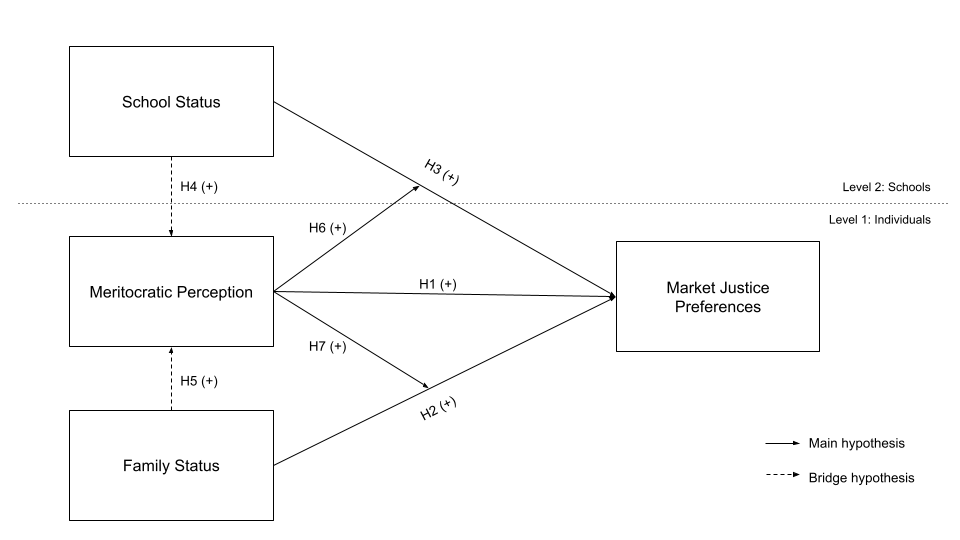
\includegraphics[width=6.25in,height=\textheight]{input/img/hypothesis2.png}

}

\caption{\label{fig-hypotheses}Summary of hypotheses}

\end{figure}%

\section{Data, Variables and Methods}\label{data-variables-and-methods}

\subsection{Data}\label{data}

The First Study of Civic Education in Chile, conducted by the Agency for
Quality Education of the Ministry of Education in 2017, is the primary
data source. This database comprises a civic knowledge test score and a
series of items that measure different aspects of citizenship. The
target population includes 8th-grade students in 242 schools nationwide.
Initially, the database contains 8,589 student observations.To ensure
higher data quality and considering the survey's unit of analysis, we
removed 171 student cases that exhibited repetitive and careless
response patterns
{[}\citeproc{ref-gottfried_autocorrelation_2022}{73}{]}. Additionally,
we utilized data from the System for Measuring the Quality of Education
(SIMCE) conducted by the Ministry of Education in 2017, which provides
school-level information such as administrative dependence,
socioeconomic classification, and results obtained in standardized
mathematics and language tests. After processing the variables and
removing missing cases, the final database for this study includes a
two-level stratified sample composed of 5,047 students (level 1) nested
within 231 schools (level 2).

\subsection{Variables}\label{variables}

\textbf{\emph{Individual level}}

\textbf{Market Justice Preferences}: The dependent variables in this
study are market justice preferences. This construct is measured through
three variables that address the degree of justification regarding
whether access to social services in pensions, education, and health
should be conditional on income. The Justification of inequality in
health is measured by the following item: ``Is it fair in Chile that
people with higher incomes can access better healthcare than those with
lower incomes?'' The same question is asked for education and pensions.
In all cases, respondents indicate their preferences on a Likert scale
ranging from ``completely disagree'' (1) to ``completely agree'' (4).
Additionally, we include a summarized indicator of ``market justice
preferences'', measured by an average index across these items (α =
0.86), with values ranging from 1 to 4, where higher values represent
stronger preferences for market justice (see
Table~\ref{tbl-desc-dependientes}). We analyzed these items
independently and by the average index.

\begin{longtable}[]{@{}
  >{\raggedright\arraybackslash}p{(\columnwidth - 6\tabcolsep) * \real{0.4286}}
  >{\raggedright\arraybackslash}p{(\columnwidth - 6\tabcolsep) * \real{0.2551}}
  >{\raggedright\arraybackslash}p{(\columnwidth - 6\tabcolsep) * \real{0.2143}}
  >{\raggedright\arraybackslash}p{(\columnwidth - 6\tabcolsep) * \real{0.1020}}@{}}
\caption{Dependent
variables}\label{tbl-desc-dependientes}\tabularnewline
\toprule\noalign{}
\begin{minipage}[b]{\linewidth}\raggedright
Label
\end{minipage} & \begin{minipage}[b]{\linewidth}\raggedright
Stats / Values
\end{minipage} & \begin{minipage}[b]{\linewidth}\raggedright
Freqs (\% of Valid)
\end{minipage} & \begin{minipage}[b]{\linewidth}\raggedright
Valid
\end{minipage} \\
\midrule\noalign{}
\endfirsthead
\toprule\noalign{}
\begin{minipage}[b]{\linewidth}\raggedright
Label
\end{minipage} & \begin{minipage}[b]{\linewidth}\raggedright
Stats / Values
\end{minipage} & \begin{minipage}[b]{\linewidth}\raggedright
Freqs (\% of Valid)
\end{minipage} & \begin{minipage}[b]{\linewidth}\raggedright
Valid
\end{minipage} \\
\midrule\noalign{}
\endhead
\bottomrule\noalign{}
\endlastfoot
It is just that in Chile people with higher incomes can have better
pensions than people with low incomes &
\begin{minipage}[t]{\linewidth}\raggedright
1. Strongly disagree\\
2. Disagree\\
3. Agree\\
4. Strongly agree\strut
\end{minipage} & \begin{minipage}[t]{\linewidth}\raggedright
1837 (30.6\%)\\
1945 (32.4\%)\\
1622 (27.0\%)\\
608 (10.1\%)\strut
\end{minipage} & \begin{minipage}[t]{\linewidth}\raggedright
6012\\
(95.9\%)\strut
\end{minipage} \\
It is just that in Chile people who can pay have a better education for
their children & \begin{minipage}[t]{\linewidth}\raggedright
1. Strongly disagree\\
2. Disagree\\
3. Agree\\
4. Strongly agree\strut
\end{minipage} & \begin{minipage}[t]{\linewidth}\raggedright
1766 (29.7\%)\\
1732 (29.1\%)\\
1704 (28.6\%)\\
750 (12.6\%)\strut
\end{minipage} & \begin{minipage}[t]{\linewidth}\raggedright
5952\\
(94.9\%)\strut
\end{minipage} \\
It is just that in Chile people with higher incomes can access better
health services than people with low incomes &
\begin{minipage}[t]{\linewidth}\raggedright
1. Strongly disagree\\
2. Disagree\\
3. Agree\\
4. Strongly agree\strut
\end{minipage} & \begin{minipage}[t]{\linewidth}\raggedright
2254 (38.0\%)\\
1685 (28.4\%)\\
1401 (23.6\%)\\
593 (10.0\%)\strut
\end{minipage} & \begin{minipage}[t]{\linewidth}\raggedright
5933\\
(94.6\%)\strut
\end{minipage} \\
Market Justice Preferences & \begin{minipage}[t]{\linewidth}\raggedright
Mean (sd) : 2.2 (0.9)\\
min \textless{} med \textless{} max:\\
1 \textless{} 2 \textless{} 4\\
IQR (CV) : 1.7 (0.4)\strut
\end{minipage} & 13 distinct values &
\begin{minipage}[t]{\linewidth}\raggedright
6077\\
(96.9\%)\strut
\end{minipage} \\
\end{longtable}

\textbf{Perception of Meritocracy}: The main independent variable refers
to the perception of meritocracy, operationalized through five items
addressing the perception of rewards based on talent and intelligence at
both the school and societal levels. At the school level, students
respond to whether ``Intelligence is important for getting good grades''
and ``Effort is important for getting good grades''. At the societal
level, students respond to the following questions: ``In Chile, people
are rewarded for their effort'', ``In Chile, people get what they
deserve'' and ``In Chile, people are rewarded for their intelligence and
skills''. Each item was answered on a four-point Likert scale ranging
from ``completely disagree'' (1) to ``completely agree'' (4).

\textbf{Family Socioeconomic Status}: The socioeconomic status of
students' families is measured using two indicators. First, the highest
educational level attained by the parents, with categories: ``8th grade
or less,'' ``Secondary education,'' ``Technical higher education,''
``University or postgraduate,'' and ``No response.'' The inclusion of
the ``No response'' category is due to its high frequency in the data;
omitting it could obscure relevant associations. Second, the number of
books in the household is used, categorized as ``Less than 25'' and
``More than 25.''

Table~\ref{tbl-desc-independent} shows the individual level variables
used, their response categories and their frequencies.

\begin{longtable}[]{@{}
  >{\raggedright\arraybackslash}p{(\columnwidth - 6\tabcolsep) * \real{0.3925}}
  >{\raggedright\arraybackslash}p{(\columnwidth - 6\tabcolsep) * \real{0.3084}}
  >{\raggedright\arraybackslash}p{(\columnwidth - 6\tabcolsep) * \real{0.1963}}
  >{\raggedright\arraybackslash}p{(\columnwidth - 6\tabcolsep) * \real{0.1028}}@{}}
\caption{Individual level
variables}\label{tbl-desc-independent}\tabularnewline
\toprule\noalign{}
\begin{minipage}[b]{\linewidth}\raggedright
Label
\end{minipage} & \begin{minipage}[b]{\linewidth}\raggedright
Stats / Values
\end{minipage} & \begin{minipage}[b]{\linewidth}\raggedright
Freqs (\% of Valid)
\end{minipage} & \begin{minipage}[b]{\linewidth}\raggedright
Valid
\end{minipage} \\
\midrule\noalign{}
\endfirsthead
\toprule\noalign{}
\begin{minipage}[b]{\linewidth}\raggedright
Label
\end{minipage} & \begin{minipage}[b]{\linewidth}\raggedright
Stats / Values
\end{minipage} & \begin{minipage}[b]{\linewidth}\raggedright
Freqs (\% of Valid)
\end{minipage} & \begin{minipage}[b]{\linewidth}\raggedright
Valid
\end{minipage} \\
\midrule\noalign{}
\endhead
\bottomrule\noalign{}
\endlastfoot
Intelligence is important to get good grades &
\begin{minipage}[t]{\linewidth}\raggedright
1. Strongly disagree\\
2. Disagree\\
3. Agree\\
4. Strongly agree\strut
\end{minipage} & \begin{minipage}[t]{\linewidth}\raggedright
367 ( 6.1\%)\\
920 (15.3\%)\\
2970 (49.4\%)\\
1760 (29.3\%)\strut
\end{minipage} & \begin{minipage}[t]{\linewidth}\raggedright
6017\\
(95.9\%)\strut
\end{minipage} \\
Effort is important to get good grades &
\begin{minipage}[t]{\linewidth}\raggedright
1. Strongly disagree\\
2. Disagree\\
3. Agree\\
4. Strongly agree\strut
\end{minipage} & \begin{minipage}[t]{\linewidth}\raggedright
109 ( 1.8\%)\\
88 ( 1.5\%)\\
1427 (23.7\%)\\
4406 (73.1\%)\strut
\end{minipage} & \begin{minipage}[t]{\linewidth}\raggedright
6030\\
(96.1\%)\strut
\end{minipage} \\
In Chile, people are rewarded for their intelligence and skill &
\begin{minipage}[t]{\linewidth}\raggedright
1. Strongly disagree\\
2. Disagree\\
3. Agree\\
4. Strongly agree\strut
\end{minipage} & \begin{minipage}[t]{\linewidth}\raggedright
517 ( 9.0\%)\\
1568 (27.3\%)\\
2673 (46.6\%)\\
983 (17.1\%)\strut
\end{minipage} & \begin{minipage}[t]{\linewidth}\raggedright
5741\\
(91.5\%)\strut
\end{minipage} \\
In Chile, people are rewarded for their efforts &
\begin{minipage}[t]{\linewidth}\raggedright
1. Strongly disagree\\
2. Disagree\\
3. Agree\\
4. Strongly agree\strut
\end{minipage} & \begin{minipage}[t]{\linewidth}\raggedright
512 ( 8.7\%)\\
1733 (29.4\%)\\
2607 (44.2\%)\\
1050 (17.8\%)\strut
\end{minipage} & \begin{minipage}[t]{\linewidth}\raggedright
5902\\
(94.1\%)\strut
\end{minipage} \\
In Chile, people get what they deserve &
\begin{minipage}[t]{\linewidth}\raggedright
1. Strongly disagree\\
2. Disagree\\
3. Agree\\
4. Strongly agree\strut
\end{minipage} & \begin{minipage}[t]{\linewidth}\raggedright
604 (10.5\%)\\
1911 (33.1\%)\\
2388 (41.4\%)\\
871 (15.1\%)\strut
\end{minipage} & \begin{minipage}[t]{\linewidth}\raggedright
5774\\
(92.1\%)\strut
\end{minipage} \\
Parental educational level & \begin{minipage}[t]{\linewidth}\raggedright
1. 8th grade or less\\
2. Secondary Education\\
3. Higher tec. education\\
4. University or Postgraduat\\
5. Missing\strut
\end{minipage} & \begin{minipage}[t]{\linewidth}\raggedright
559 ( 8.9\%)\\
1698 (27.1\%)\\
960 (15.3\%)\\
1080 (17.2\%)\\
1975 (31.5\%)\strut
\end{minipage} & \begin{minipage}[t]{\linewidth}\raggedright
6272\\
(100.0\%)\strut
\end{minipage} \\
Number of books at home & \begin{minipage}[t]{\linewidth}\raggedright
1. Les than 25\\
2. More than 25\strut
\end{minipage} & \begin{minipage}[t]{\linewidth}\raggedright
3920 (63.2\%)\\
2281 (36.8\%)\strut
\end{minipage} & \begin{minipage}[t]{\linewidth}\raggedright
6201\\
(98.9\%)\strut
\end{minipage} \\
\end{longtable}

\textbf{\emph{Contextual level}}

This study focuses on two school-level characteristics: socioeconomic
status and academic performance. Socioeconomic status is assessed using
the Ministry of Education's classification, measured as an ordinal item
with five categories ranging from ``low'' (1) to ``high'' (5). Academic
performance is measured using the school's results in the SIMCE (System
of Measurement of Educational Quality) standardized tests, administered
yearly at different educational levels in language and mathematics.
These results are categorized as ``low,'' ``medium,'' and ``high.'' The
contextual level items used, response categories, and their frequencies
are detailed in Table~\ref{tbl-desc-school}.

\begin{longtable}[]{@{}
  >{\raggedright\arraybackslash}p{(\columnwidth - 6\tabcolsep) * \real{0.4138}}
  >{\raggedright\arraybackslash}p{(\columnwidth - 6\tabcolsep) * \real{0.2184}}
  >{\raggedright\arraybackslash}p{(\columnwidth - 6\tabcolsep) * \real{0.2414}}
  >{\raggedright\arraybackslash}p{(\columnwidth - 6\tabcolsep) * \real{0.1264}}@{}}
\caption{School context variables}\label{tbl-desc-school}\tabularnewline
\toprule\noalign{}
\begin{minipage}[b]{\linewidth}\raggedright
Label
\end{minipage} & \begin{minipage}[b]{\linewidth}\raggedright
Stats / Values
\end{minipage} & \begin{minipage}[b]{\linewidth}\raggedright
Freqs (\% of Valid)
\end{minipage} & \begin{minipage}[b]{\linewidth}\raggedright
Valid
\end{minipage} \\
\midrule\noalign{}
\endfirsthead
\toprule\noalign{}
\begin{minipage}[b]{\linewidth}\raggedright
Label
\end{minipage} & \begin{minipage}[b]{\linewidth}\raggedright
Stats / Values
\end{minipage} & \begin{minipage}[b]{\linewidth}\raggedright
Freqs (\% of Valid)
\end{minipage} & \begin{minipage}[b]{\linewidth}\raggedright
Valid
\end{minipage} \\
\midrule\noalign{}
\endhead
\bottomrule\noalign{}
\endlastfoot
Socioeconomic level of school &
\begin{minipage}[t]{\linewidth}\raggedright
1. Low\\
2. Medium low\\
3. Medium\\
4. Medium high\\
5. High\strut
\end{minipage} & \begin{minipage}[t]{\linewidth}\raggedright
49 (21.1\%)\\
92 (39.7\%)\\
43 (18.5\%)\\
29 (12.5\%)\\
19 ( 8.2\%)\strut
\end{minipage} & \begin{minipage}[t]{\linewidth}\raggedright
232\\
(100.0\%)\strut
\end{minipage} \\
SIMCE score achievement by school &
\begin{minipage}[t]{\linewidth}\raggedright
1. Low\\
2. Medium\\
3. High\strut
\end{minipage} & \begin{minipage}[t]{\linewidth}\raggedright
108 (46.6\%)\\
69 (29.7\%)\\
55 (23.7\%)\strut
\end{minipage} & \begin{minipage}[t]{\linewidth}\raggedright
232\\
(100.0\%)\strut
\end{minipage} \\
\end{longtable}

\textbf{\emph{Controls}}

A series of control variables are included. At the individual level, an
index of access to technology is constructed based on the number of
computers, tablets, and cell phones in the household, as well as
internet connectivity. At the contextual level, we use the
administrative dependence of schools, classified as ``Public,''
``Subsidized Private,'' or ``Private,'' and the proportion of parents
with university or postgraduate education at each school.

\subsection{Methods}\label{methods}

Given the hierarchical structure of the data, with students nested
within schools, model estimation is performed within a multilevel
framework. These models are appropriate for capturing both individual
and contextual effects in a single analysis, allowing for the estimation
of fixed effects between groups and random effects that vary from one
group to another
{[}\citeproc{ref-bell_fixed_2019}{74},\citeproc{ref-hox_multilevel_2010}{75}{]}.
Cumulative link mixed models were employed for the ordinal dependent
variables, while linear mixed-effects models were applied for the
average market justice preference index.

The hypotheses of this research were pre-registered in the Open Science
Framework platform of the Center for Open Science (OSF), and access to
the document is available at this
\href{https://doi.org/10.17605/OSF.IO/UFSDV}{link}. The statistical
analysis for this research was conducted using the \emph{lme4} package
in R version 4.1.3.

\section{Results}\label{results}

\subsection{Descriptive statistics}\label{descriptive-statistics}

Figure~\ref{fig-marketjustice} illustrates the distribution of responses
to the three items on market justice preferences (healthcare, pensions,
and education), indicating that most respondents tend to disagree or
strongly disagree with the idea that it is just for people with higher
incomes to have access to better services in these areas. The strongest
opposition is observed in the healthcare sector, as the majority of
respondents (66.4\%) are against the idea that higher-income individuals
should have access to better healthcare services. Similarly, regarding
the concept of justice related to access to better pensions based on
income, the level of disagreement reaches 63.0\%. This decreases
significantly in the field of education, as the percentage of
respondents who disagree or strongly disagree with those with higher
incomes having access to better education decreases to 58.8\%. Only a
small proportion agree that access to healthcare should be conditional
on income (23.6\%), and a minority strongly agree (10\%), as is the case
with pensions. However, this increases in the case of education, being
the area where there is a significant proportion of respondents who
agree or strongly agree with access based on market justice (41.2\%).

\begin{figure}

\centering{

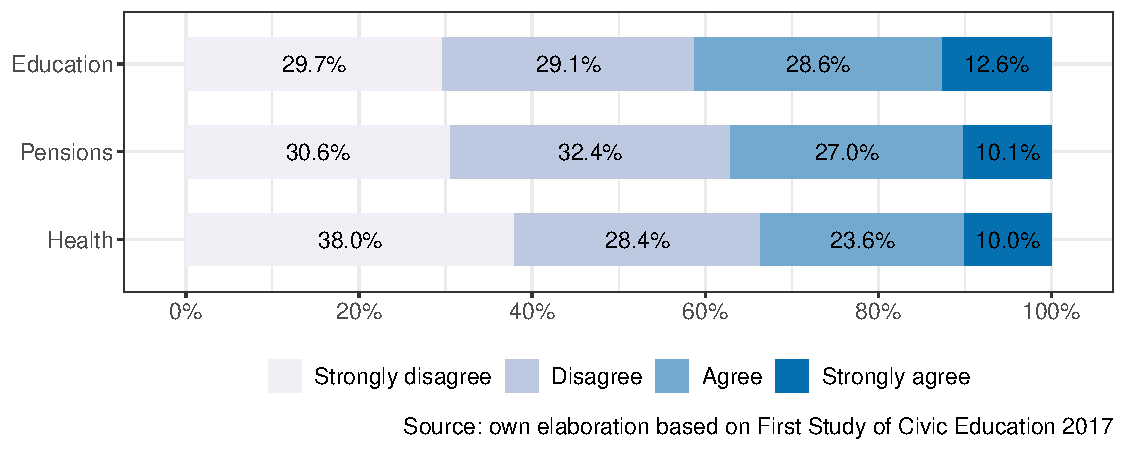
\includegraphics{paper-blinded_files/figure-pdf/fig-marketjustice-1.pdf}

}

\caption{\label{fig-marketjustice}Market justice preferences in health,
pensions and education}

\end{figure}%

Regarding the perception of meritocracy, Figure~\ref{fig-meritocracy}
displays the frequency distribution of five items related to the
dimensions of school and society. At the school level, there is a strong
belief that both effort and talent are important for achieving good
grades, with especially high agreement for effort. Specifically, while
78.6\% agree or strongly agree on the importance of talent for obtaining
good grades, this proportion rises to 96.8\% for effort, indicating that
respondents value effort more than talent in this context.

\begin{figure}

\centering{

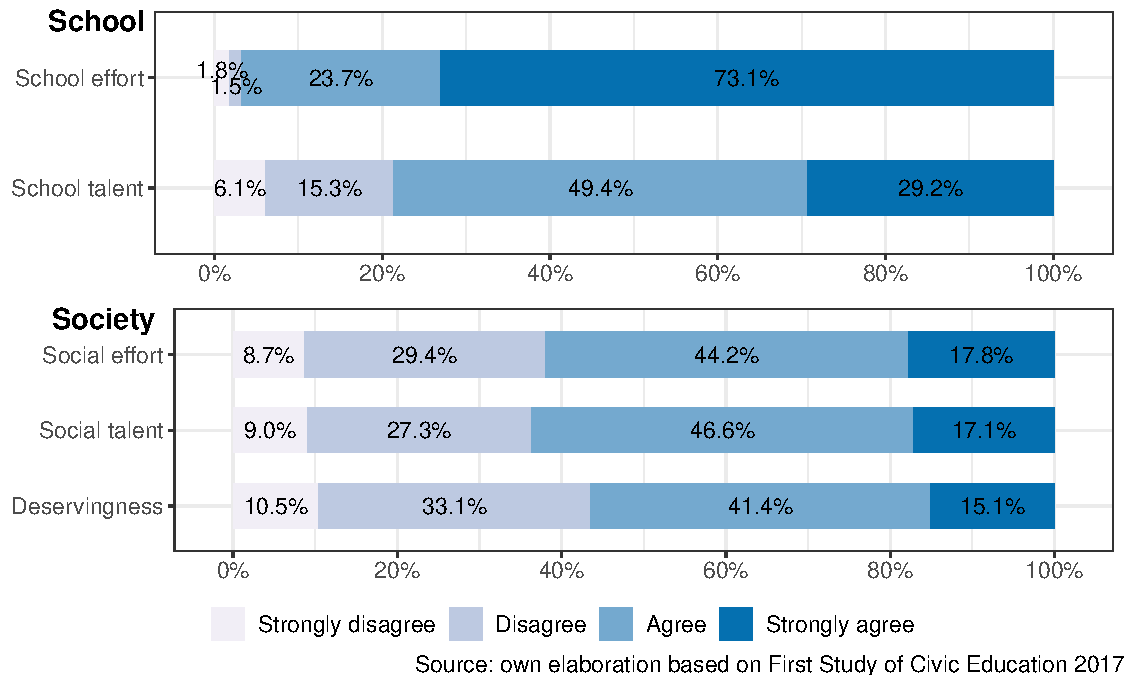
\includegraphics{paper-blinded_files/figure-pdf/fig-meritocracy-1.pdf}

}

\caption{\label{fig-meritocracy}Social and school meritocracy}

\end{figure}%

At the societal level, Figure~\ref{fig-meritocracy} shows that a
majority of respondents agree or strongly agree that individuals are
rewarded for their talents (63.7\%) and efforts (62\%). Nevertheless, a
notable proportion perceives that both effort and talent are not
adequately rewarded in society, with 38.1\% and 36.3\% respectively. The
perception of whether people get what they deserve in society is more
divided; while a slim majority (56.5\% combining agree and strongly
agree) agrees, a significant minority (43.6\%) disagrees, indicating
that this is the most contentious item among respondents. There is
general agreement that people are rewarded for talent and effort in
society, but the consensus is weaker compared to school meritocracy.

Figure~\ref{fig-bivariate} shows a series of graphs depicting the
association between the variables of market justice preferences - in
education, health, and pensions - and the variables of meritocratic
perception at school (effort and talent) and in society (effort, talent,
and deservingness) (see conceptual diagram in
Figure~\ref{fig-hypotheses}). In general we observe a positive
association between meritocracy and market justice preferences for the
societal questions, but this is not as straightforward for the school
items, particularly for the one referred to effort.

\begin{figure}

\centering{

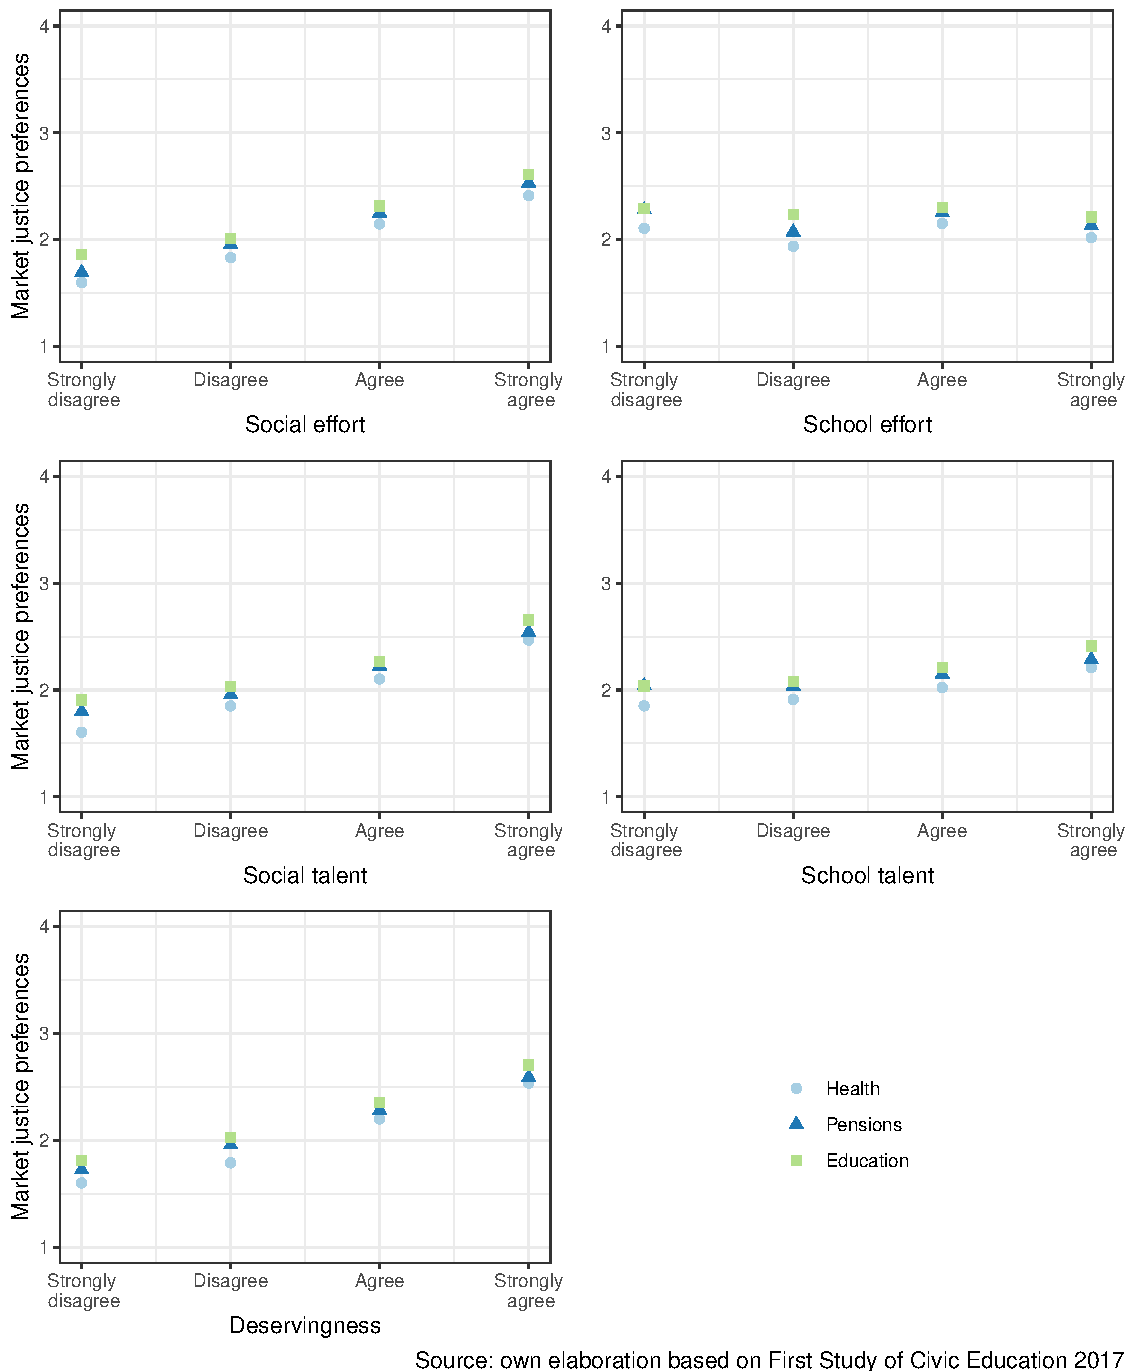
\includegraphics{paper-blinded_files/figure-pdf/fig-bivariate-1.pdf}

}

\caption{\label{fig-bivariate}Market justice preferences in education,
health and pensions by social and school meritocracy}

\end{figure}%

\subsection{Multivariate analysis}\label{multivariate-analysis}

This section presents the results of the multilevel models. We begin by
showing the results of the cumulative link mixed models in
Table~\ref{tbl-ordinal-reg} for the ordinal dependent variables of
justice in health, pensions, and education separately in order to
compare the effect of the predictors. Then, we present the results of
the linear mixed-effects models for the average index of preference for
market justice in Table~\ref{tbl-lineal-reg}\footnote{The table shows
  the effects of individual and contextual-level independent variables
  related to our hypotheses; however, the models also incorporate the
  control variables for each of the three dependent variables separately
  and for the average index (complete models are available in the
  \hyperref[appendix]{Supplementary Material}).}.

For the health item, the intraclass correlation (ICC) obtained for the
null model (not shown) indicates that 5\% of the total variance of this
item is associated with specific characteristics of the schools, while
it is 3\% for the pensions item and 4\% for the education item {[}ICC
based on \citeproc{ref-hox_multilevel_2010}{75}{]}. For the average
index of market justice preferences, the ICC reaches 4\%, indicating
that overall, only a small percentage of the total variance in students'
market justice preferences is associated with school characteristics,
thus limiting the possibility of finding effects at this second level of
analysis.

\begin{table}

\caption{\label{tbl-ordinal-reg}Cumulative link multilevel models of
differential acces justificacion of health, pensions, and education}

\centering{

\begin{center}
\scalebox{0.8}{
\begin{threeparttable}
\begin{tabular}{l c c c c c c}
\toprule
 & \multicolumn{2}{c}{Health} & \multicolumn{2}{c}{Pensions} & \multicolumn{2}{c}{Education} \\
\cmidrule(lr){2-3} \cmidrule(lr){4-5} \cmidrule(lr){6-7}
 & Model 1 & Model 2 & Model 1 & Model 2 & Model 1 & Model 2 \\
\midrule
School talent                             & $0.23^{***}$  & $0.22^{***}$  & $0.17^{***}$  & $0.16^{***}$  & $0.25^{***}$  & $0.25^{***}$  \\
                                          & $(0.03)$      & $(0.03)$      & $(0.03)$      & $(0.03)$      & $(0.03)$      & $(0.03)$      \\
School effort                             & $-0.26^{***}$ & $-0.26^{***}$ & $-0.26^{***}$ & $-0.25^{***}$ & $-0.23^{***}$ & $-0.23^{***}$ \\
                                          & $(0.04)$      & $(0.04)$      & $(0.04)$      & $(0.04)$      & $(0.04)$      & $(0.04)$      \\
Social talent                             & $0.16^{***}$  & $0.16^{***}$  & $0.12^{**}$   & $0.13^{**}$   & $0.14^{**}$   & $0.15^{***}$  \\
                                          & $(0.05)$      & $(0.05)$      & $(0.04)$      & $(0.04)$      & $(0.04)$      & $(0.04)$      \\
Social effort                             & $0.11^{*}$    & $0.11^{*}$    & $0.27^{***}$  & $0.27^{***}$  & $0.15^{**}$   & $0.15^{**}$   \\
                                          & $(0.05)$      & $(0.05)$      & $(0.05)$      & $(0.05)$      & $(0.05)$      & $(0.05)$      \\
Deservingness                             & $0.52^{***}$  & $0.51^{***}$  & $0.38^{***}$  & $0.37^{***}$  & $0.44^{***}$  & $0.43^{***}$  \\
                                          & $(0.05)$      & $(0.05)$      & $(0.05)$      & $(0.05)$      & $(0.05)$      & $(0.05)$      \\
Parental education (Ref.= Non-university) &               &               &               &               &               &               \\
                                          &               &               &               &               &               &               \\
\quad University or posgraduate           & $0.05$        & $0.08$        & $0.14$        & $0.12$        & $0.09$        & $0.07$        \\
                                          & $(0.08)$      & $(0.08)$      & $(0.08)$      & $(0.08)$      & $(0.08)$      & $(0.08)$      \\
\quad Missing                             & $0.10$        & $0.11$        & $0.12^{*}$    & $0.11$        & $0.13^{*}$    & $0.12^{*}$    \\
                                          & $(0.06)$      & $(0.06)$      & $(0.06)$      & $(0.06)$      & $(0.06)$      & $(0.06)$      \\
More than 25 books (Ref.= Less than 25)   & $-0.16^{**}$  & $-0.13^{*}$   & $-0.13^{*}$   & $-0.13^{*}$   & $-0.07$       & $-0.07$       \\
                                          & $(0.06)$      & $(0.06)$      & $(0.06)$      & $(0.06)$      & $(0.06)$      & $(0.06)$      \\
Socioeconomic level (Ref.= Low)           &               &               &               &               &               &               \\
                                          &               &               &               &               &               &               \\
\quad SES Medium                          &               & $0.08$        &               & $0.02$        &               & $0.08$        \\
                                          &               & $(0.10)$      &               & $(0.10)$      &               & $(0.10)$      \\
\quad SES High                            &               & $0.71^{*}$    &               & $0.72^{**}$   &               & $0.93^{***}$  \\
                                          &               & $(0.28)$      &               & $(0.26)$      &               & $(0.28)$      \\
Achievement score (Ref.= Low)             &               &               &               &               &               &               \\
                                          &               &               &               &               &               &               \\
\quad Simce Medium                        &               & $-0.29^{***}$ &               & $-0.19^{*}$   &               & $-0.16^{*}$   \\
                                          &               & $(0.08)$      &               & $(0.08)$      &               & $(0.08)$      \\
\quad Simce High                          &               & $-0.56^{***}$ &               & $-0.53^{***}$ &               & $-0.46^{***}$ \\
                                          &               & $(0.10)$      &               & $(0.09)$      &               & $(0.10)$      \\
\midrule
Controls                                  & Yes           & Yes           & Yes           & Yes           & Yes           & Yes           \\
BIC                                       & $12747.58$    & $12761.47$    & $13103.81$    & $13112.87$    & $13329.33$    & $13352.18$    \\
Num.obs                                   & $5144$        & $5144$        & $5177$        & $5177$        & $5159$        & $5159$        \\
Num. groups: Schools                      & $231$         & $231$         & $232$         & $232$         & $231$         & $231$         \\
Var: Schools (Intercept)                  & $0.11$        & $0.05$        & $0.09$        & $0.04$        & $0.10$        & $0.05$        \\
\bottomrule
\end{tabular}
\begin{tablenotes}[flushleft]
\scriptsize{\item Note: Cells contain regression coefficients with standard errors in parentheses. Control variables are included. $^{***}p<0.001$; $^{**}p<0.01$; $^{*}p<0.05$ \\ \item Source: own elaboration based on First Study of Civic Education 2017.}
\end{tablenotes}
\end{threeparttable}
}
\caption{}
\label{table:coefficients}
\end{center}

}

\end{table}%

Model 1 in Table~\ref{tbl-ordinal-reg} for the three dependent variables
of justice in differential access to health, pensions, and education
demonstrates a similar trend regarding the effect of the perception of
meritocracy on these items, with all effects being statistically
significant (\emph{p} \textless{} 0.05). Regarding the variables of
social meritocracy, the three variables---talent (\(\beta\) = 0.16),
effort (\(\beta\) = 0.11), and deservingness (\(\beta\) = 0.51)---show
that as these increase, the justification for differentiated access to
pensions, education, and health also increases. In the context of school
meritocracy, the effects are mixed: as perceived school talent
increases, the justification for differentiated access to these services
increases (\(\beta\) = 0.23); conversely, as perceived school effort
increases, the justification decreases (\(\beta\) = -0.26), holding all
other variables constant.

Additionally, Model 1 examines family status through parents'
educational level and the number of books at home. For health, pensions,
and education, a negative but statistically non-significant association
with parents' education is observed. However, having more than 25 books
at home shows a negative and statistically significant effect on market
justice in health and pensions (\(\beta\) = -0.13; \emph{p} \textless{}
0.001), suggesting less justification for differentiated access compared
to those with fewer books.

Model 2 in Table~\ref{tbl-ordinal-reg} incorporates school-level
variables. The results show that high socioeconomic level schools show
greater preferences for market justice in health, pensions, and
education compared to low socioeconomic level schools, with
statistically significant results (\(\beta\) = 0.71; \emph{p}
\textless{} 0.05). Moreover, and contrary to our hypothesis, schools
with higher academic performance show negative and statistically
significant effects across the three items (\(\beta\) = -0.56; \emph{p}
\textless{} 0.001).

\begin{table}

\caption{\label{tbl-lineal-reg}Linear mixed-effects models for
meritocracy perception and market justice preferences}

\centering{

\begin{center}
\scalebox{0.85}{
\begin{threeparttable}
\begin{tabular}{l c c c c}
\toprule
 & Model 1 & Model 2 & Model 3 & Model 4 \\
\midrule
Constant                                  & $1.31^{***}$  & $1.30^{***}$  & $1.36^{***}$  & $1.39^{***}$  \\
                                          & $(0.09)$      & $(0.10)$      & $(0.10)$      & $(0.10)$      \\
School talent                             & $0.11^{***}$  & $0.11^{***}$  & $0.10^{***}$  & $0.10^{***}$  \\
                                          & $(0.01)$      & $(0.01)$      & $(0.01)$      & $(0.01)$      \\
School effort                             & $-0.12^{***}$ & $-0.12^{***}$ & $-0.12^{***}$ & $-0.12^{***}$ \\
                                          & $(0.02)$      & $(0.02)$      & $(0.02)$      & $(0.02)$      \\
Social talent                             & $0.07^{***}$  & $0.07^{***}$  & $0.07^{***}$  & $0.07^{***}$  \\
                                          & $(0.02)$      & $(0.02)$      & $(0.02)$      & $(0.02)$      \\
Social effort                             & $0.08^{***}$  & $0.08^{***}$  & $0.08^{***}$  & $0.08^{***}$  \\
                                          & $(0.02)$      & $(0.02)$      & $(0.02)$      & $(0.02)$      \\
Deservingness                             & $0.20^{***}$  & $0.20^{***}$  & $0.20^{***}$  & $0.20^{***}$  \\
                                          & $(0.02)$      & $(0.02)$      & $(0.02)$      & $(0.02)$      \\
Parental education (Ref.= Non-university) &               &               &               &               \\
                                          &               &               &               &               \\
\quad University or posgraduate           &               & $0.05$        & $0.05$        & $0.05$        \\
                                          &               & $(0.03)$      & $(0.04)$      & $(0.04)$      \\
\quad Missing                             &               & $0.06^{*}$    & $0.06^{*}$    & $0.06^{*}$    \\
                                          &               & $(0.03)$      & $(0.03)$      & $(0.03)$      \\
More than 25 books (Ref.= Less than 25)   &               & $-0.05$       & $-0.05$       & $-0.04$       \\
                                          &               & $(0.03)$      & $(0.03)$      & $(0.03)$      \\
Socioeconomic level (Ref.= Low)           &               &               &               &               \\
                                          &               &               &               &               \\
\quad SES Medium                          &               &               & $-0.01$       & $0.01$        \\
                                          &               &               & $(0.05)$      & $(0.05)$      \\
\quad SES High                            &               &               & $0.31^{*}$    & $0.37^{**}$   \\
                                          &               &               & $(0.14)$      & $(0.13)$      \\
Achievement score (Ref.= Low)             &               &               &               &               \\
                                          &               &               &               &               \\
\quad Simce Medium                        &               &               &               & $-0.11^{**}$  \\
                                          &               &               &               & $(0.04)$      \\
\quad Simce High                          &               &               &               & $-0.26^{***}$ \\
                                          &               &               &               & $(0.04)$      \\
\midrule
Controls                                  & Yes           & Yes           & Yes           & Yes           \\
Deviance                                  & $12368.01$    & $12359.40$    & $12344.10$    & $12310.90$    \\
Deviance Test (p)                         & $0.00$        & $0.00$        & $0.00$        & $0.00$        \\
BIC                                       & $12517.46$    & $12550.41$    & $12595.11$    & $12589.48$    \\
Num.obs                                   & $5047$        & $5047$        & $5047$        & $5047$        \\
Num. groups: Schools                      & $231$         & $231$         & $231$         & $231$         \\
Var: Schools (Intercept)                  & $0.02$        & $0.02$        & $0.02$        & $0.01$        \\
Var: Residual                             & $0.66$        & $0.66$        & $0.67$        & $0.66$        \\
\bottomrule
\end{tabular}
\begin{tablenotes}[flushleft]
\scriptsize{\item Note: Cells contain regression coefficients with standard errors in parentheses. Control variables are included. $^{***}p<0.001$; $^{**}p<0.01$; $^{*}p<0.05$ \\ \item Source: own elaboration based on First Study of Civic Education 2017.}
\end{tablenotes}
\end{threeparttable}
}
\caption{}
\label{table:coefficients}
\end{center}

}

\end{table}%

Table~\ref{tbl-lineal-reg} ppresents the results of linear mixed-effects
models for the market justice preference index. Model 1 shows that
higher perceived societal meritocracy, through effort (\(\beta\) =
0.08), talent (\(\beta\) = 0.07), and deservingness (\(\beta\) = 0.2),
is positively and significantly associated with market justice
preferences (\emph{p} \textless{} 0.001). School meritocracy perceptions
yield mixed effects: perceived talent increases market justice
preference (\(\beta\) = 0.1), while perceived effort decreases it
(\(\beta\) = -0.12), both statistically significant (\emph{p}
\textless{} 0.001). Model 2 includes family status, finding no
statistically significant effects from parents' education or the number
of books at home. Regarding school characteristics, Models 3 and 4
introduce socioeconomic level and academic performance. The results of
Model 3 suggest a statistically significant relationship between school
socioeconomic levels and market justice preferences, specifically those
schools with high socioeconomic levels (\(\beta\) = 0.37; \emph{p}
\textless{} 0.01) compared to low socioeconomic levels. However, Model 4
indicates that schools with medium (\(\beta\) = -0.11; \emph{p}
\textless{} 0.01) and high (\(\beta\) = -0.26; \emph{p} \textless{}
0.001) academic performance present lower market justice preferences
compared to low-performing schools, with these effects being
statistically significant when controlling for other variables.

\begin{table}

\caption{\label{tbl-interact}Interactions effects}

\centering{

\resizebox{\linewidth}{!}{
\begin{tabu} to \linewidth {>{\raggedright\arraybackslash}p{4cm}>{\centering\arraybackslash}p{1.5cm}>{\centering\arraybackslash}p{1.5cm}>{\centering\arraybackslash}p{1.5cm}>{\centering\arraybackslash}p{1.5cm}>{\centering\arraybackslash}p{1.5cm}}
\toprule
\multicolumn{1}{c}{\textbf{ }} & \multicolumn{5}{c}{\textbf{Market Justice Preferences}} \\
\cmidrule(l{3pt}r{3pt}){2-6}
Variable & School talent & School effort & Social talent & Social effort & Deservingness\\
\midrule
\textbf{University or Postgraduate} & -0.034 & -0.012 & -0.073. & -0.079* & -0.118**\\
\cmidrule{1-6}
\textbf{More than 25 books} & -0.015 & -0.046 & -0.029 & -0.081** & -0.035\\
\cmidrule{1-6}
\textbf{School SES high} & 0.004 & 0.001 & -0.057. & -0.063* & -0.08**\\
\cmidrule{1-6}
\textbf{Simce Medium} & 0.001 & 0.032 & -0.037 & -0.041 & -0.082*\\
\cmidrule{1-6}
\textbf{Simce High} & -0.016 & 0.008 & -0.043 & -0.063. & -0.087*\\
\bottomrule
\multicolumn{6}{l}{\textsuperscript{} Note: ***p < 0.001, **p < 0.01, *p < 0.05. Source: own elaboration based on First Study of Civic}\\
\multicolumn{6}{l}{Education 2017.}\\
\end{tabu}}

}

\end{table}%

Table~\ref{tbl-interact} displays the interaction terms related to our
hypotheses. The results suggest that students' family background
moderates the relationship between their meritocratic perceptions and
their justification of market allocation in social services.
Specifically, the relationship between social effort and market justice
preferences is less positive for students whose parents have university
or postgraduate education (\(\beta\) = -0.079; \emph{p} \textless{}
0.05). Lower-status students (measured by parental education) prefer
more market justice when they strongly adhere to meritocratic
perceptions of deservingness (\(\beta\) = -0.118; \emph{p} \textless{}
0.01). A similar moderating effect is seen with family cultural capital:
the relationship between effort and market justice preferences is less
positive for students with more than 25 books at home (\(\beta\) =
-0.081; \emph{p} \textless{} 0.01).

At the school level, we observe that school status and students'
meritocratic beliefs moderate their preferences for market justice.
High-status schools show less preference for market justice when their
students, on average, have a greater perception of meritocracy, as
measured by effort, deservingness, and talent. Conversely, low-achieving
schools prefer more market justice when their students have stronger
meritocratic beliefs. Figure~\ref{fig-interaction} illustrates this
moderating effect of school achievement on the relationship between
deservingness and market justice. No moderating effects were observed at
the school level for students' meritocratic beliefs regarding effort or
talent in achieving good grades.

\begin{figure}

\centering{

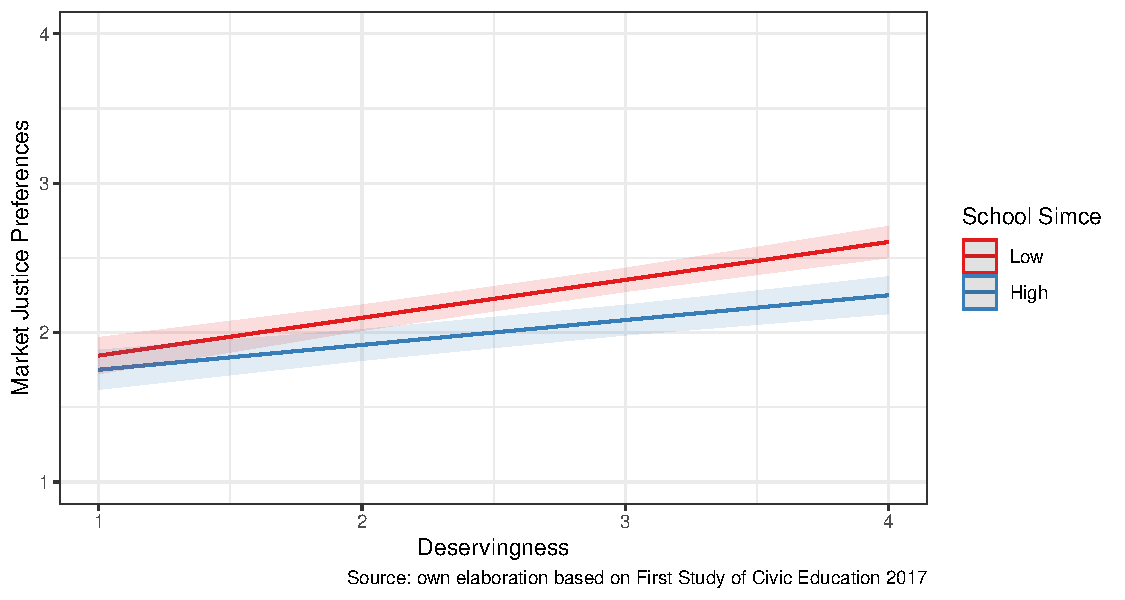
\includegraphics{paper-blinded_files/figure-pdf/fig-interaction-1.pdf}

}

\caption{\label{fig-interaction}Interaction between deservingness and
justification of inequality by school SIMCE achievement}

\end{figure}%

\section{Discussion}\label{discussion}

The previous analyses aimed to explore the relationship between
perceptions of meritocracy and preferences for market justice among
students in Chilean society. Several models estimated how students'
beliefs about the rewards for talent and effort in both societal and
school contexts influence their attitudes toward access to social
services like health, education, and pensions based on pay capacity.
Additionally, the models examined the impact of students' socioeconomic
status and school achievement on these preferences, assessing whether
perceptions of meritocracy moderate these effects. The findings offer
insights into the complex interplay between meritocratic beliefs,
socioeconomic factors, and attitudes toward market justice criteria.

Hypothesis \(H_{1a}\) posited that students who perceive greater
meritocracy in society would show stronger preferences for market
justice. The results support this hypothesis, indicating a positive
relationship between the perception that talent and effort are rewarded
in society and the preferences for market justice in access to services
such as health, education, and pensions. This finding aligns with
previous research suggesting that individuals who believe in a
meritocratic system are more likely to justify social inequalities
{[}\citeproc{ref-batruch_belief_2022}{3},\citeproc{ref-wiederkehr_belief_2015}{4}{]}.
It is noteworthy that among the items measuring meritocratic perception,
consistently the one about deservingness shows a larger effect when
compared to the ones about talent and effort. Although the three items
correlate, there is something distinctive about deservingness that
probably encompasses other aspects beyond meritocracy, an aspect to
which we will come back in the conclusions. Moving now to hypothesis
\(H_{1b}\), this is simply a variation of 1a, replacing the perception
of meritocracy at society by the one at school. In this case we have
only two items of meritocratic perception - unfortunately deservingness
was not measured at school level - and the direction of the effects is
not as straightforward as in the case of societal meritocracy in
\(H_{1a}\): positive for talent, but negative for effort. Still, one of
the limitation for the comparison between perception of meritocracy and
society is the difference of the items' phrasing. Whereas for society
the item refers to the extent to which efforts are rewarded, at school
is about the importance of effort, whereby something that is important
does not necessarily mean that it is enough to be rewarded. Furthermore,
the school-effort item is the one with the lowest variation among all
meritocratic items (more than 95\% agree or strongly agree), and with
the lowest effect size.

Hypothesis \(H_2\) and hypothesis \(H_3\) propose that socioeconomic
status could influence students' preferences, but the results show
different patterns. On the one hand, \(H_2\) proposed that students from
higher socioeconomic status families would show stronger preferences for
market justice, which is not supported by the results. Although students
from families with higher educational levels and more economic resources
tend to prefer less market justice, this relationship is not
statistically significant. This might be due to the influence of other
contextual and cultural factors that modulate attitudes toward market
justice
{[}\citeproc{ref-kohn_social_1963}{66},\citeproc{ref-kohn_class_1969}{67},\citeproc{ref-almas_fairness_2017}{70}{]}.
Notably, socioeconomic status measured by parental educational level and
the number of books at home do not explain variations in market justice
preferences, suggesting that other variables, such as market justice
preferences of parents, could play an essential role in the attitudinal
socialization process. On the other hand, Hypothesis \(H_3\) held that
students from schools with higher socioeconomic status would show
stronger preferences for market justice. The results confirm this
hypothesis since students from high-status schools tend to prefer more
market justice, compared to low-status schools. This finding, in line
with the existing literature
{[}\citeproc{ref-jonsson_institutional_2015}{71},\citeproc{ref-jost_attitudinal_2000}{72}{]},
does allow us to affirm the hypothesis about the role of the school
environment, particularly socioeconomic segregation, in influencing
attitudes towards market justice and the acceptance of inequalities. A
possible explanation is the role of the context at the school level,
which could have a more relevant role than the family socioeconomic
status, since the highly stratified nature of the Chilean education
system reinforces socioeconomic divisions and socializes students into
different normative frameworks.

Hypothesis \(H_4\) held that students from schools with higher school
achievement would show stronger preferences for market justice,
following the argument that such schools could foster meritocratic
attitudes by showing a larger promotion of talent and effort in order to
get better results. Nevertheless, the results show quite the opposite:
schools with better academic results (as measured by a national
standardized test) show in average less preferences for market justice.
This finding is one of the most strongest and consistent throughout the
models and it is relevant given the centrality of school performance in
educational institutions. One possible explanation of this link is that
students in high-achieving schools may be more exposed to discussions
and a deeper understanding of inequality and social justice, leading to
a critical perspective toward the weight of market mechanisms in the
access to social services.

Hypotheses \(H_5\) and \(H_6\) proposed that socioeconomic status would
moderate the effect of meritocratic perceptions on market justice
preferences. Hypothesis \(H_5\) refers to family socioeconomic status,
whereby the results show a negative interaction with two of the three
perceptual variables at the societal level. This means that the positive
impact of the perception of social meritocracy on market justice
preferences had a lower effect on students with parents with higher
education and also on those with more books at home. Something similar
occurs with hypothesis \(H_6\), where now school-level status moderates
the effect of meritocracy variables, which in multilevel framework is
referred as to cross-level interaction. The negative interaction in this
context means that in schools of low socioeconomic levels, the positive
effect of the social meritocracy variables on market justice preferences
is stronger. These relations indicate that, although those who perceive
society as meritocratic have greater preferences towards market justice,
this influence is lower among those with a higher socioeconomic level.
This finding highlights the complex interaction between socioeconomic
status, school context, meritocratic beliefs, and preferences toward
market justice. The moderating role of meritocratic perceptions suggests
that students' views on social justice are shaped by their socioeconomic
background and beliefs about how society rewards effort and talent. This
underlines the importance of addressing structural inequalities and
individual beliefs in educational and social policies.

Hypothesis \(H7\) posited that the academic performance of schools could
moderate the effect of meritocratic perceptions on preferences for
market justice. This hypothesis is based on the argument that the level
of academic performance in schools entails a differentiated promotion of
meritocratic perceptions to achieve better results, which would, in
turn, reinforce or diminish preferences for market justice. The results
of the interactions between levels suggest that, indeed, in
higher-performing schools, the effect of meritocratic perceptions on the
justification of service provision based on market principles is weaker
compared to lower-performing schools. Similarly to the effect of
academic performance in \(H4\), a possible explanation for this
moderation is that students in high-performing schools may be more
exposed to knowledge about the effects of inequality and social justice.
This exposure translates into an enlightening effect of education on
inequality, which can mitigate the impact of meritocracy on market
justice preferences.

\section{Conclusion}\label{conclusion}

Our research aimed to examine the relationship between the perception of
meritocracy and the justification of market justice preferences among
eighth-grade students in Chile. From our knowledge this is the first
study addressing market justice preferences at school level, finding
that students exhibit large preferences for market justice (about one
third agree or strongly agree with them), a share that is quite larger
when compared with evidence in adult population. Perception of
meritocracy is also high, particularly when it comes to the reward of
effort, with an striking eighty six percent of agreement. Regarding
these descriptive indicators, a a first message coming from this study
is that there is something particular in school-age when it comes to
perceptions and preferences about inequality. This can relate to
development aspects {[}\citeproc{ref-rizzo_children_2020}{77}{]} but it
could be something specific to the Chilean case, which requires further
comparative as well as longitudinal research in the area. In any case,
teaching about the origins and characteristics of social inequality is
not part of the chilean school curriculum, calling for a more dedicated
consideration of these topics in areas such as citizensip education as
well as in history and social science education.

The core of this paper was the association between meritocratic
perceptions and preferences for market justice. In general, we find that
those who perceive that effort and talent/intelligence are rewarded, are
more willing to agree with that richer individuals can have better
health, education, and pensions. This is not the first time that
meritocratic perceptions (and also beliefs) have been related with the
legitimation of social inequalities
{[}\citeproc{ref-mijs_paradox_2019}{51},\citeproc{ref-darnon_where_2018}{63}{]},
but the consideration of school level population as well as market
justice preferences allows adding evidence regarding the role of
meritocracy regarding inequality beliefs: legitimation of market
criteria in social services seems to begin at school age, and what
students think of meritocracy is linked to it. Although there are still
several open questions, as for instance differences between meritocratic
perceptions in school and in the society at large, this raises up the
relevance of what is done (or not) in schools in order to challenge the
meritocratic ideals.

The consideration of the school context opened some caveats in this
research. We found contrary evidence for the association between status,
school performance, and market justice preferences: high status and high
achievement at the school level are associated with less market justice
preferences. This is opposed to the rational-interest argument that
suggests that those doing better - both economically and academically-
would demand less redistribution
{[}\citeproc{ref-bullock_education_2021}{80}{]} and therefore are
expected to challenge market mechanisms. A possible explanation is that
education contributes to forming a critical view of markets in
redistribution, nevertheless, further research in this area is needed to
assert the specific mechanisms that might be playing a role. All in all,
from this study we know that school contexts are not trivial in this
regard, calling for larger attention to school-age research on the
formation of inequality preferences and beliefs.

\newpage{}

\section{Supplementary material}\label{supplementary-material}

\subsection{Complete multilevel
models}\label{complete-multilevel-models}

\begin{table}

\caption{\label{tbl-ordinal-health}Cumulative Link Multilevel Models for
Justifying Differential Access to Health Care}

\centering{

\begin{center}
\scalebox{0.7}{
\begin{threeparttable}
\begin{tabular}{l c c c c c c}
\toprule
 & Model 0 & Model 1 & Model 2 & Model 3 & Model 4 & Model 5 \\
\midrule
Strongly Disagree|Disagree                             & $-0.55^{***}$ & $1.23^{***}$  & $1.20^{***}$  & $1.24^{***}$  & $1.05^{***}$  & $1.04^{***}$  \\
                                                       & $(0.04)$      & $(0.20)$      & $(0.20)$      & $(0.22)$      & $(0.23)$      & $(0.23)$      \\
Disagree|Agree                                         & $0.68^{***}$  & $2.54^{***}$  & $2.52^{***}$  & $2.55^{***}$  & $2.37^{***}$  & $2.36^{***}$  \\
                                                       & $(0.04)$      & $(0.20)$      & $(0.20)$      & $(0.22)$      & $(0.24)$      & $(0.24)$      \\
Agree|Strongly Agree                                   & $2.25^{***}$  & $4.20^{***}$  & $4.18^{***}$  & $4.22^{***}$  & $4.03^{***}$  & $4.02^{***}$  \\
                                                       & $(0.06)$      & $(0.21)$      & $(0.21)$      & $(0.23)$      & $(0.24)$      & $(0.24)$      \\
School talent                                          &               & $0.23^{***}$  & $0.23^{***}$  & $0.23^{***}$  & $0.22^{***}$  & $0.22^{***}$  \\
                                                       &               & $(0.03)$      & $(0.03)$      & $(0.03)$      & $(0.03)$      & $(0.03)$      \\
School effort                                          &               & $-0.27^{***}$ & $-0.26^{***}$ & $-0.26^{***}$ & $-0.26^{***}$ & $-0.26^{***}$ \\
                                                       &               & $(0.04)$      & $(0.04)$      & $(0.04)$      & $(0.04)$      & $(0.04)$      \\
Social talent                                          &               & $0.16^{***}$  & $0.16^{***}$  & $0.16^{***}$  & $0.16^{***}$  & $0.16^{***}$  \\
                                                       &               & $(0.05)$      & $(0.05)$      & $(0.05)$      & $(0.05)$      & $(0.05)$      \\
Social effort                                          &               & $0.11^{*}$    & $0.11^{*}$    & $0.11^{*}$    & $0.11^{*}$    & $0.11^{*}$    \\
                                                       &               & $(0.05)$      & $(0.05)$      & $(0.05)$      & $(0.05)$      & $(0.05)$      \\
Deservingness                                          &               & $0.52^{***}$  & $0.52^{***}$  & $0.52^{***}$  & $0.51^{***}$  & $0.51^{***}$  \\
                                                       &               & $(0.05)$      & $(0.05)$      & $(0.05)$      & $(0.05)$      & $(0.05)$      \\
Parental education (Ref.= Non-university)              &               &               &               &               &               &               \\
                                                       &               &               &               &               &               &               \\
\quad University or posgraduate                        &               &               & $0.05$        & $0.05$        & $0.06$        & $0.08$        \\
                                                       &               &               & $(0.08)$      & $(0.08)$      & $(0.08)$      & $(0.08)$      \\
\quad Missing                                          &               &               & $0.10$        & $0.10$        & $0.10$        & $0.11$        \\
                                                       &               &               & $(0.06)$      & $(0.06)$      & $(0.06)$      & $(0.06)$      \\
More than 25 books (Ref.= Less than 25)                &               &               & $-0.16^{**}$  & $-0.16^{**}$  & $-0.14^{*}$   & $-0.13^{*}$   \\
                                                       &               &               & $(0.06)$      & $(0.06)$      & $(0.06)$      & $(0.06)$      \\
Technology acces                                       &               &               &               & $0.00$        & $0.00$        & $0.00$        \\
                                                       &               &               &               & $(0.01)$      & $(0.01)$      & $(0.01)$      \\
No internet connectivity (Ref.= Internet connectivity) &               &               &               & $0.03$        & $0.01$        & $-0.00$       \\
                                                       &               &               &               & $(0.06)$      & $(0.07)$      & $(0.07)$      \\
Socioeconomic level (Ref.= Low)                        &               &               &               &               &               &               \\
                                                       &               &               &               &               &               &               \\
\quad SES Medium                                       &               &               &               &               & $0.04$        & $0.08$        \\
                                                       &               &               &               &               & $(0.10)$      & $(0.10)$      \\
\quad SES High                                         &               &               &               &               & $0.48^{**}$   & $0.71^{*}$    \\
                                                       &               &               &               &               & $(0.16)$      & $(0.28)$      \\
Achievement score (Ref.= Low)                          &               &               &               &               &               &               \\
                                                       &               &               &               &               &               &               \\
\quad Simce Medium                                     &               &               &               &               & $-0.31^{***}$ & $-0.29^{***}$ \\
                                                       &               &               &               &               & $(0.08)$      & $(0.08)$      \\
\quad Simce High                                       &               &               &               &               & $-0.61^{***}$ & $-0.56^{***}$ \\
                                                       &               &               &               &               & $(0.09)$      & $(0.10)$      \\
Prop. university level at school                       &               &               &               &               &               & $-0.34$       \\
                                                       &               &               &               &               &               & $(0.36)$      \\
School dependence (Ref.= Public)                       &               &               &               &               &               &               \\
                                                       &               &               &               &               &               &               \\
\quad Subsidized Private                               &               &               &               &               &               & $-0.05$       \\
                                                       &               &               &               &               &               & $(0.08)$      \\
\quad Private                                          &               &               &               &               &               & $-0.14$       \\
                                                       &               &               &               &               &               & $(0.27)$      \\
\midrule
Log Likelihood                                         & $-6581.84$    & $-6314.90$    & $-6309.98$    & $-6309.70$    & $-6287.72$    & $-6286.73$    \\
AIC                                                    & $13171.69$    & $12647.80$    & $12643.95$    & $12649.39$    & $12613.44$    & $12617.47$    \\
BIC                                                    & $13197.87$    & $12706.71$    & $12722.50$    & $12747.58$    & $12737.80$    & $12761.47$    \\
Num.obs                                                & $5144$        & $5144$        & $5144$        & $5144$        & $5144$        & $5144$        \\
Num. groups: Schools                                   & $231$         & $231$         & $231$         & $231$         & $231$         & $231$         \\
Var: Schools (Intercept)                               & $0.17$        & $0.11$        & $0.11$        & $0.11$        & $0.05$        & $0.05$        \\
\bottomrule
\end{tabular}
\begin{tablenotes}[flushleft]
\scriptsize{\item Note: Cells contain regression coefficients with standard errors in parentheses. $^{***}p<0.001$; $^{**}p<0.01$; $^{*}p<0.05$ \\ \item Source: own elaboration based on First Study of Civic Education 2017.}
\end{tablenotes}
\end{threeparttable}
}
\caption{}
\label{table:coefficients}
\end{center}

}

\end{table}%

\begin{table}

\caption{\label{tbl-ordinal-pension}Cumulative Link Multilevel Models
for Justifying Differential Access to Pensions}

\centering{

\begin{center}
\scalebox{0.7}{
\begin{threeparttable}
\begin{tabular}{l c c c c c c}
\toprule
 & Model 0 & Model 1 & Model 2 & Model 3 & Model 4 & Model 5 \\
\midrule
Strongly Disagree|Disagree                             & $-0.89^{***}$ & $0.69^{***}$  & $0.71^{***}$  & $0.85^{***}$  & $0.67^{**}$   & $0.67^{**}$   \\
                                                       & $(0.04)$      & $(0.20)$      & $(0.20)$      & $(0.22)$      & $(0.23)$      & $(0.23)$      \\
Disagree|Agree                                         & $0.52^{***}$  & $2.18^{***}$  & $2.21^{***}$  & $2.35^{***}$  & $2.17^{***}$  & $2.17^{***}$  \\
                                                       & $(0.04)$      & $(0.20)$      & $(0.20)$      & $(0.22)$      & $(0.23)$      & $(0.23)$      \\
Agree|Strongly Agree                                   & $2.25^{***}$  & $4.01^{***}$  & $4.03^{***}$  & $4.18^{***}$  & $4.00^{***}$  & $4.00^{***}$  \\
                                                       & $(0.05)$      & $(0.21)$      & $(0.21)$      & $(0.22)$      & $(0.24)$      & $(0.24)$      \\
School talent                                          &               & $0.17^{***}$  & $0.17^{***}$  & $0.17^{***}$  & $0.16^{***}$  & $0.16^{***}$  \\
                                                       &               & $(0.03)$      & $(0.03)$      & $(0.03)$      & $(0.03)$      & $(0.03)$      \\
School effort                                          &               & $-0.25^{***}$ & $-0.25^{***}$ & $-0.26^{***}$ & $-0.25^{***}$ & $-0.25^{***}$ \\
                                                       &               & $(0.04)$      & $(0.04)$      & $(0.04)$      & $(0.04)$      & $(0.04)$      \\
Social talent                                          &               & $0.13^{**}$   & $0.12^{**}$   & $0.12^{**}$   & $0.13^{**}$   & $0.13^{**}$   \\
                                                       &               & $(0.04)$      & $(0.04)$      & $(0.04)$      & $(0.04)$      & $(0.04)$      \\
Social effort                                          &               & $0.27^{***}$  & $0.27^{***}$  & $0.27^{***}$  & $0.27^{***}$  & $0.27^{***}$  \\
                                                       &               & $(0.05)$      & $(0.05)$      & $(0.05)$      & $(0.05)$      & $(0.05)$      \\
Deservingness                                          &               & $0.38^{***}$  & $0.38^{***}$  & $0.38^{***}$  & $0.37^{***}$  & $0.37^{***}$  \\
                                                       &               & $(0.05)$      & $(0.05)$      & $(0.05)$      & $(0.05)$      & $(0.05)$      \\
Parental education (Ref.= Non-university)              &               &               &               &               &               &               \\
                                                       &               &               &               &               &               &               \\
\quad University or posgraduate                        &               &               & $0.16^{*}$    & $0.14$        & $0.12$        & $0.12$        \\
                                                       &               &               & $(0.08)$      & $(0.08)$      & $(0.08)$      & $(0.08)$      \\
\quad Missing                                          &               &               & $0.13^{*}$    & $0.12^{*}$    & $0.11$        & $0.11$        \\
                                                       &               &               & $(0.06)$      & $(0.06)$      & $(0.06)$      & $(0.06)$      \\
More than 25 books (Ref.= Less than 25)                &               &               & $-0.12^{*}$   & $-0.13^{*}$   & $-0.13^{*}$   & $-0.13^{*}$   \\
                                                       &               &               & $(0.06)$      & $(0.06)$      & $(0.06)$      & $(0.06)$      \\
Technology acces                                       &               &               &               & $0.02^{*}$    & $0.02$        & $0.02$        \\
                                                       &               &               &               & $(0.01)$      & $(0.01)$      & $(0.01)$      \\
No internet connectivity (Ref.= Internet connectivity) &               &               &               & $-0.01$       & $-0.03$       & $-0.03$       \\
                                                       &               &               &               & $(0.06)$      & $(0.06)$      & $(0.06)$      \\
Socioeconomic level (Ref.= Low)                        &               &               &               &               &               &               \\
                                                       &               &               &               &               &               &               \\
\quad SES Medium                                       &               &               &               &               & $0.00$        & $0.02$        \\
                                                       &               &               &               &               & $(0.10)$      & $(0.10)$      \\
\quad SES High                                         &               &               &               &               & $0.69^{***}$  & $0.72^{**}$   \\
                                                       &               &               &               &               & $(0.15)$      & $(0.26)$      \\
Achievement score (Ref.= Low)                          &               &               &               &               &               &               \\
                                                       &               &               &               &               &               &               \\
\quad Simce Medium                                     &               &               &               &               & $-0.21^{**}$  & $-0.19^{*}$   \\
                                                       &               &               &               &               & $(0.07)$      & $(0.08)$      \\
\quad Simce High                                       &               &               &               &               & $-0.53^{***}$ & $-0.53^{***}$ \\
                                                       &               &               &               &               & $(0.08)$      & $(0.09)$      \\
Prop. university level at school                       &               &               &               &               &               & $0.22$        \\
                                                       &               &               &               &               &               & $(0.34)$      \\
School dependence (Ref.= Public)                       &               &               &               &               &               &               \\
                                                       &               &               &               &               &               &               \\
\quad Subsidized Private                               &               &               &               &               &               & $-0.09$       \\
                                                       &               &               &               &               &               & $(0.07)$      \\
\quad Private                                          &               &               &               &               &               & $-0.15$       \\
                                                       &               &               &               &               &               & $(0.25)$      \\
\midrule
Log Likelihood                                         & $-6737.05$    & $-6494.86$    & $-6490.03$    & $-6487.76$    & $-6463.24$    & $-6462.36$    \\
AIC                                                    & $13482.11$    & $13007.72$    & $13004.05$    & $13005.53$    & $12964.49$    & $12968.73$    \\
BIC                                                    & $13508.31$    & $13066.68$    & $13082.68$    & $13103.81$    & $13088.98$    & $13112.87$    \\
Num.obs                                                & $5177$        & $5177$        & $5177$        & $5177$        & $5177$        & $5177$        \\
Num. groups: Schools                                   & $232$         & $232$         & $232$         & $232$         & $232$         & $232$         \\
Var: Schools (Intercept)                               & $0.11$        & $0.09$        & $0.09$        & $0.09$        & $0.04$        & $0.04$        \\
\bottomrule
\end{tabular}
\begin{tablenotes}[flushleft]
\scriptsize{\item Note: Cells contain regression coefficients with standard errors in parentheses. $^{***}p<0.001$; $^{**}p<0.01$; $^{*}p<0.05$ \\ \item Source: own elaboration based on First Study of Civic Education 2017.}
\end{tablenotes}
\end{threeparttable}
}
\caption{}
\label{table:coefficients}
\end{center}

}

\end{table}%

\begin{table}

\caption{\label{tbl-ordinal-educ}Cumulative Link Multilevel Models for
Justifying Differential Access to Education}

\centering{

\begin{center}
\scalebox{0.7}{
\begin{threeparttable}
\begin{tabular}{l c c c c c c}
\toprule
 & Model 0 & Model 1 & Model 2 & Model 3 & Model 4 & Model 5 \\
\midrule
Strongly Disagree|Disagree                             & $-0.93^{***}$ & $0.84^{***}$  & $0.87^{***}$  & $0.82^{***}$  & $0.75^{**}$   & $0.75^{**}$   \\
                                                       & $(0.04)$      & $(0.20)$      & $(0.20)$      & $(0.22)$      & $(0.23)$      & $(0.23)$      \\
Disagree|Agree                                         & $0.34^{***}$  & $2.19^{***}$  & $2.23^{***}$  & $2.18^{***}$  & $2.11^{***}$  & $2.11^{***}$  \\
                                                       & $(0.04)$      & $(0.20)$      & $(0.20)$      & $(0.22)$      & $(0.23)$      & $(0.23)$      \\
Agree|Strongly Agree                                   & $1.98^{***}$  & $3.93^{***}$  & $3.96^{***}$  & $3.92^{***}$  & $3.85^{***}$  & $3.85^{***}$  \\
                                                       & $(0.05)$      & $(0.20)$      & $(0.21)$      & $(0.22)$      & $(0.24)$      & $(0.24)$      \\
School talent                                          &               & $0.25^{***}$  & $0.25^{***}$  & $0.25^{***}$  & $0.25^{***}$  & $0.25^{***}$  \\
                                                       &               & $(0.03)$      & $(0.03)$      & $(0.03)$      & $(0.03)$      & $(0.03)$      \\
School effort                                          &               & $-0.24^{***}$ & $-0.23^{***}$ & $-0.23^{***}$ & $-0.23^{***}$ & $-0.23^{***}$ \\
                                                       &               & $(0.04)$      & $(0.04)$      & $(0.04)$      & $(0.04)$      & $(0.04)$      \\
Social talent                                          &               & $0.14^{**}$   & $0.14^{**}$   & $0.14^{**}$   & $0.15^{***}$  & $0.15^{***}$  \\
                                                       &               & $(0.04)$      & $(0.04)$      & $(0.04)$      & $(0.04)$      & $(0.04)$      \\
Social effort                                          &               & $0.15^{**}$   & $0.15^{**}$   & $0.15^{**}$   & $0.15^{**}$   & $0.15^{**}$   \\
                                                       &               & $(0.05)$      & $(0.05)$      & $(0.05)$      & $(0.05)$      & $(0.05)$      \\
Deservingness                                          &               & $0.44^{***}$  & $0.44^{***}$  & $0.44^{***}$  & $0.43^{***}$  & $0.43^{***}$  \\
                                                       &               & $(0.05)$      & $(0.05)$      & $(0.05)$      & $(0.05)$      & $(0.05)$      \\
Parental education (Ref.= Non-university)              &               &               &               &               &               &               \\
                                                       &               &               &               &               &               &               \\
\quad University or posgraduate                        &               &               & $0.09$        & $0.09$        & $0.06$        & $0.07$        \\
                                                       &               &               & $(0.08)$      & $(0.08)$      & $(0.08)$      & $(0.08)$      \\
\quad Missing                                          &               &               & $0.13^{*}$    & $0.13^{*}$    & $0.12^{*}$    & $0.12^{*}$    \\
                                                       &               &               & $(0.06)$      & $(0.06)$      & $(0.06)$      & $(0.06)$      \\
More than 25 books (Ref.= Less than 25)                &               &               & $-0.07$       & $-0.07$       & $-0.07$       & $-0.07$       \\
                                                       &               &               & $(0.06)$      & $(0.06)$      & $(0.06)$      & $(0.06)$      \\
Technology acces                                       &               &               &               & $-0.00$       & $-0.01$       & $-0.01$       \\
                                                       &               &               &               & $(0.01)$      & $(0.01)$      & $(0.01)$      \\
No internet connectivity (Ref.= Internet connectivity) &               &               &               & $-0.04$       & $-0.04$       & $-0.05$       \\
                                                       &               &               &               & $(0.06)$      & $(0.06)$      & $(0.06)$      \\
Socioeconomic level (Ref.= Low)                        &               &               &               &               &               &               \\
                                                       &               &               &               &               &               &               \\
\quad SES Medium                                       &               &               &               &               & $0.08$        & $0.08$        \\
                                                       &               &               &               &               & $(0.10)$      & $(0.10)$      \\
\quad SES High                                         &               &               &               &               & $0.75^{***}$  & $0.93^{***}$  \\
                                                       &               &               &               &               & $(0.16)$      & $(0.28)$      \\
Achievement score (Ref.= Low)                          &               &               &               &               &               &               \\
                                                       &               &               &               &               &               &               \\
\quad Simce Medium                                     &               &               &               &               & $-0.16^{*}$   & $-0.16^{*}$   \\
                                                       &               &               &               &               & $(0.08)$      & $(0.08)$      \\
\quad Simce High                                       &               &               &               &               & $-0.47^{***}$ & $-0.46^{***}$ \\
                                                       &               &               &               &               & $(0.09)$      & $(0.10)$      \\
Prop. university level at school                       &               &               &               &               &               & $-0.17$       \\
                                                       &               &               &               &               &               & $(0.35)$      \\
School dependence (Ref.= Public)                       &               &               &               &               &               &               \\
                                                       &               &               &               &               &               &               \\
\quad Subsidized Private                               &               &               &               &               &               & $0.04$        \\
                                                       &               &               &               &               &               & $(0.08)$      \\
\quad Private                                          &               &               &               &               &               & $-0.14$       \\
                                                       &               &               &               &               &               & $(0.27)$      \\
\midrule
Log Likelihood                                         & $-6846.16$    & $-6603.77$    & $-6600.80$    & $-6600.55$    & $-6582.51$    & $-6582.06$    \\
AIC                                                    & $13700.33$    & $13225.55$    & $13225.60$    & $13231.10$    & $13203.03$    & $13208.12$    \\
BIC                                                    & $13726.52$    & $13284.48$    & $13304.18$    & $13329.33$    & $13327.45$    & $13352.18$    \\
Num.obs                                                & $5159$        & $5159$        & $5159$        & $5159$        & $5159$        & $5159$        \\
Num. groups: Schools                                   & $231$         & $231$         & $231$         & $231$         & $231$         & $231$         \\
Var: Schools (Intercept)                               & $0.13$        & $0.10$        & $0.10$        & $0.10$        & $0.05$        & $0.05$        \\
\bottomrule
\end{tabular}
\begin{tablenotes}[flushleft]
\scriptsize{\item Note: Cells contain regression coefficients with standard errors in parentheses. $^{***}p<0.001$; $^{**}p<0.01$; $^{*}p<0.05$ \\ \item Source: own elaboration based on First Study of Civic Education 2017.}
\end{tablenotes}
\end{threeparttable}
}
\caption{}
\label{table:coefficients}
\end{center}

}

\end{table}%

\begin{table}

\caption{\label{tbl-lineal-reg-complete}Linear mixed-effects models for
meritocracy perception and market justice preferences}

\centering{

\begin{center}
\scalebox{0.7}{
\begin{threeparttable}
\begin{tabular}{l c c c c c c}
\toprule
 & Model 0 & Model 1 & Model 2 & Model 3 & Model 4 & Model 5 \\
\midrule
Constant                                               & $2.17^{***}$ & $1.34^{***}$  & $1.33^{***}$  & $1.30^{***}$  & $1.38^{***}$  & $1.39^{***}$  \\
                                                       & $(0.02)$     & $(0.09)$      & $(0.09)$      & $(0.10)$      & $(0.10)$      & $(0.10)$      \\
School talent                                          &              & $0.11^{***}$  & $0.11^{***}$  & $0.11^{***}$  & $0.10^{***}$  & $0.10^{***}$  \\
                                                       &              & $(0.01)$      & $(0.01)$      & $(0.01)$      & $(0.01)$      & $(0.01)$      \\
School effort                                          &              & $-0.12^{***}$ & $-0.12^{***}$ & $-0.12^{***}$ & $-0.12^{***}$ & $-0.12^{***}$ \\
                                                       &              & $(0.02)$      & $(0.02)$      & $(0.02)$      & $(0.02)$      & $(0.02)$      \\
Social talent                                          &              & $0.07^{***}$  & $0.07^{***}$  & $0.07^{***}$  & $0.07^{***}$  & $0.07^{***}$  \\
                                                       &              & $(0.02)$      & $(0.02)$      & $(0.02)$      & $(0.02)$      & $(0.02)$      \\
Social effort                                          &              & $0.08^{***}$  & $0.08^{***}$  & $0.08^{***}$  & $0.08^{***}$  & $0.08^{***}$  \\
                                                       &              & $(0.02)$      & $(0.02)$      & $(0.02)$      & $(0.02)$      & $(0.02)$      \\
Deservingness                                          &              & $0.20^{***}$  & $0.20^{***}$  & $0.20^{***}$  & $0.20^{***}$  & $0.20^{***}$  \\
                                                       &              & $(0.02)$      & $(0.02)$      & $(0.02)$      & $(0.02)$      & $(0.02)$      \\
Parental education (Ref.= Non-university)              &              &               &               &               &               &               \\
                                                       &              &               &               &               &               &               \\
\quad University or posgraduate                        &              &               & $0.05$        & $0.05$        & $0.04$        & $0.05$        \\
                                                       &              &               & $(0.03)$      & $(0.03)$      & $(0.04)$      & $(0.04)$      \\
\quad Missing                                          &              &               & $0.06^{*}$    & $0.06^{*}$    & $0.06^{*}$    & $0.06^{*}$    \\
                                                       &              &               & $(0.03)$      & $(0.03)$      & $(0.03)$      & $(0.03)$      \\
More than 25 books (Ref.= Less than 25)                &              &               & $-0.05$       & $-0.05$       & $-0.04$       & $-0.04$       \\
                                                       &              &               & $(0.03)$      & $(0.03)$      & $(0.03)$      & $(0.03)$      \\
Technology acces                                       &              &               &               & $0.00$        & $0.00$        & $0.00$        \\
                                                       &              &               &               & $(0.01)$      & $(0.01)$      & $(0.01)$      \\
No internet connectivity (Ref.= Internet connectivity) &              &               &               & $0.00$        & $-0.01$       & $-0.01$       \\
                                                       &              &               &               & $(0.03)$      & $(0.03)$      & $(0.03)$      \\
Socioeconomic level (Ref.= Low)                        &              &               &               &               &               &               \\
                                                       &              &               &               &               &               &               \\
\quad SES Medium                                       &              &               &               &               & $0.01$        & $0.01$        \\
                                                       &              &               &               &               & $(0.04)$      & $(0.05)$      \\
\quad SES High                                         &              &               &               &               & $0.29^{***}$  & $0.37^{**}$   \\
                                                       &              &               &               &               & $(0.07)$      & $(0.13)$      \\
Achievement score (Ref.= Low)                          &              &               &               &               &               &               \\
                                                       &              &               &               &               &               &               \\
\quad Simce Medium                                     &              &               &               &               & $-0.12^{***}$ & $-0.11^{**}$  \\
                                                       &              &               &               &               & $(0.04)$      & $(0.04)$      \\
\quad Simce High                                       &              &               &               &               & $-0.27^{***}$ & $-0.26^{***}$ \\
                                                       &              &               &               &               & $(0.04)$      & $(0.04)$      \\
School dependence (Ref.= Public)                       &              &               &               &               &               &               \\
                                                       &              &               &               &               &               &               \\
\quad Prop. university level at school                 &              &               &               &               &               & $-0.05$       \\
                                                       &              &               &               &               &               & $(0.16)$      \\
\quad Subsidized Private                               &              &               &               &               &               & $-0.01$       \\
                                                       &              &               &               &               &               & $(0.04)$      \\
\quad Private                                          &              &               &               &               &               & $-0.08$       \\
                                                       &              &               &               &               &               & $(0.13)$      \\
\midrule
AIC                                                    & $12967.40$   & $12422.86$    & $12436.31$    & $12459.04$    & $12437.84$    & $12452.43$    \\
BIC                                                    & $12986.98$   & $12475.07$    & $12508.10$    & $12550.41$    & $12555.32$    & $12589.48$    \\
Log Likelihood                                         & $-6480.70$   & $-6203.43$    & $-6207.16$    & $-6215.52$    & $-6200.92$    & $-6205.21$    \\
Num.obs                                                & $5047$       & $5047$        & $5047$        & $5047$        & $5047$        & $5047$        \\
Num. groups: Schools                                   & $231$        & $231$         & $231$         & $231$         & $231$         & $231$         \\
Var: Schools (Intercept)                               & $0.03$       & $0.02$        & $0.02$        & $0.02$        & $0.01$        & $0.01$        \\
Var: Residual                                          & $0.74$       & $0.66$        & $0.66$        & $0.66$        & $0.66$        & $0.66$        \\
\bottomrule
\end{tabular}
\begin{tablenotes}[flushleft]
\scriptsize{\item Note: Cells contain regression coefficients with standard errors in parentheses. $^{***}p<0.001$; $^{**}p<0.01$; $^{*}p<0.05$ \\ \item Source: own elaboration based on First Study of Civic Education 2017.}
\end{tablenotes}
\end{threeparttable}
}
\caption{}
\label{table:coefficients}
\end{center}

}

\end{table}%

\begin{table}

\caption{\label{tbl-interac-educparent}Linear mixed-effects models for
meritocracy perception, parental education and market justice
preferences}

\centering{

\begin{center}
\scalebox{0.7}{
\begin{threeparttable}
\begin{tabular}{l c c c c c}
\toprule
 & Model 1 & Model 2 & Model 3 & Model 4 & Model 5 \\
\midrule
Constant                                            & $1.35^{***}$  & $1.31^{***}$  & $1.34^{***}$  & $1.37^{***}$  & $1.38^{***}$  \\
                                                    & $(0.10)$      & $(0.10)$      & $(0.10)$      & $(0.12)$      & $(0.10)$      \\
School talent                                       & $0.10^{***}$  & $0.10^{***}$  & $0.10^{***}$  & $0.10^{***}$  & $0.11^{***}$  \\
                                                    & $(0.01)$      & $(0.01)$      & $(0.01)$      & $(0.01)$      & $(0.02)$      \\
School effort                                       & $-0.12^{***}$ & $-0.12^{***}$ & $-0.12^{***}$ & $-0.12^{***}$ & $-0.12^{***}$ \\
                                                    & $(0.02)$      & $(0.02)$      & $(0.02)$      & $(0.03)$      & $(0.02)$      \\
Social talent                                       & $0.07^{***}$  & $0.08^{***}$  & $0.09^{***}$  & $0.08^{***}$  & $0.08^{***}$  \\
                                                    & $(0.02)$      & $(0.02)$      & $(0.02)$      & $(0.02)$      & $(0.02)$      \\
Social effort                                       & $0.09^{***}$  & $0.08^{***}$  & $0.08^{***}$  & $0.08^{***}$  & $0.08^{***}$  \\
                                                    & $(0.02)$      & $(0.02)$      & $(0.02)$      & $(0.02)$      & $(0.02)$      \\
Deservingness                                       & $0.20^{***}$  & $0.22^{***}$  & $0.20^{***}$  & $0.20^{***}$  & $0.20^{***}$  \\
                                                    & $(0.02)$      & $(0.02)$      & $(0.02)$      & $(0.02)$      & $(0.02)$      \\
Parental education (Ref.= Non-university)           &               &               &               &               &               \\
                                                    &               &               &               &               &               \\
\quad University or posgraduate                     & $0.26^{*}$    & $0.35^{***}$  & $0.25^{*}$    & $0.10$        & $0.15$        \\
                                                    & $(0.11)$      & $(0.10)$      & $(0.11)$      & $(0.23)$      & $(0.12)$      \\
\quad Missing                                       & $0.03$        & $0.13$        & $0.07$        & $0.08$        & $0.03$        \\
                                                    & $(0.09)$      & $(0.09)$      & $(0.09)$      & $(0.16)$      & $(0.10)$      \\
More than 25 books (Ref.= Less than 25)             & $-0.04$       & $-0.04$       & $-0.04$       & $-0.04$       & $-0.04$       \\
                                                    & $(0.03)$      & $(0.03)$      & $(0.03)$      & $(0.03)$      & $(0.03)$      \\
SES High (Ref.= Low)                                & $-0.06$       & $-0.06$       & $-0.06$       & $-0.06$       & $-0.06$       \\
                                                    & $(0.06)$      & $(0.05)$      & $(0.05)$      & $(0.05)$      & $(0.05)$      \\
Achievement score (Ref.= Low)                       &               &               &               &               &               \\
                                                    &               &               &               &               &               \\
\quad Simce Medium                                  & $-0.11^{**}$  & $-0.12^{***}$ & $-0.12^{***}$ & $-0.12^{***}$ & $-0.12^{***}$ \\
                                                    & $(0.04)$      & $(0.03)$      & $(0.03)$      & $(0.03)$      & $(0.03)$      \\
\quad Simce High                                    & $-0.24^{***}$ & $-0.24^{***}$ & $-0.24^{***}$ & $-0.24^{***}$ & $-0.24^{***}$ \\
                                                    & $(0.05)$      & $(0.04)$      & $(0.04)$      & $(0.04)$      & $(0.04)$      \\
Parental education x Meritocracy                    &               &               &               &               &               \\
                                                    &               &               &               &               &               \\
\quad University or posgraduate * Social effort     & $-0.08^{*}$   &               &               &               &               \\
                                                    & $(0.04)$      &               &               &               &               \\
\quad Missing * Social effort                       & $0.01$        &               &               &               &               \\
                                                    & $(0.03)$      &               &               &               &               \\
\quad University or posgraduate * Deservingness     &               & $-0.12^{**}$  &               &               &               \\
                                                    &               & $(0.04)$      &               &               &               \\
\quad Missing * Deservingness                       &               & $-0.02$       &               &               &               \\
                                                    &               & $(0.03)$      &               &               &               \\
\quad University or posgraduate * Social talent     &               &               & $-0.07$       &               &               \\
                                                    &               &               & $(0.04)$      &               &               \\
\quad Missing * Social talent                       &               &               & $0.00$        &               &               \\
                                                    &               &               & $(0.03)$      &               &               \\
\quad University or posgraduate * School effort     &               &               &               & $-0.01$       &               \\
                                                    &               &               &               & $(0.06)$      &               \\
\quad Missing * School effort                       &               &               &               & $-0.00$       &               \\
                                                    &               &               &               & $(0.04)$      &               \\
\quad University or posgraduate * School talent     &               &               &               &               & $-0.03$       \\
                                                    &               &               &               &               & $(0.04)$      \\
\quad Missing * School talent                       &               &               &               &               & $0.01$        \\
                                                    &               &               &               &               & $(0.03)$      \\
\midrule
Controls                                            & Yes           & Yes           & Yes           & Yes           & Yes           \\
AIC                                                 & $12472.82$    & $12480.94$    & $12486.54$    & $12489.10$    & $12489.36$    \\
BIC                                                 & $12649.03$    & $12657.15$    & $12662.76$    & $12665.31$    & $12665.57$    \\
Log Likelihood                                      & $-6209.41$    & $-6213.47$    & $-6216.27$    & $-6217.55$    & $-6217.68$    \\
Num.obs                                             & $5047$        & $5047$        & $5047$        & $5047$        & $5047$        \\
Num. groups: Schools                                & $231$         & $231$         & $231$         & $231$         & $231$         \\
Var: Schools (Intercept)                            & $0.01$        & $0.00$        & $0.00$        & $0.00$        & $0.00$        \\
Var: Schools University or Postgraduate             & $0.00$        & $0.01$        & $0.02$        & $0.02$        & $0.02$        \\
Var: Schools Missing                                & $0.00$        & $0.02$        & $0.02$        & $0.02$        & $0.02$        \\
Cov: Schools (Intercept) University or Postgraduate & $0.00$        & $0.00$        & $0.00$        & $0.00$        & $0.00$        \\
Cov: Schools (Intercept) Missing                    & $0.00$        & $0.00$        & $0.00$        & $0.00$        & $0.00$        \\
Cov: Schools University or Postgraduate, Missing    & $0.00$        & $0.02$        & $0.02$        & $0.02$        & $0.02$        \\
Var: Residual                                       & $0.66$        & $0.67$        & $0.67$        & $0.67$        & $0.67$        \\
\bottomrule
\end{tabular}
\begin{tablenotes}[flushleft]
\scriptsize{\item Note: Cells contain regression coefficients with standard errors in parentheses. Control variables are included. $^{***}p<0.001$; $^{**}p<0.01$; $^{*}p<0.05$ \\ \item Source: own elaboration based on First Study of Civic Education 2017.}
\end{tablenotes}
\end{threeparttable}
}
\caption{}
\label{table:coefficients}
\end{center}

}

\end{table}%

\begin{table}

\caption{\label{tbl-interac-books}Linear mixed-effects models for
meritocracy perception, books at home and market justice preferences}

\centering{

\begin{center}
\scalebox{0.7}{
\begin{threeparttable}
\begin{tabular}{l c c c c c}
\toprule
 & Model 1 & Model 2 & Model 3 & Model 4 & Model 5 \\
\midrule
Constant                                    & $1.29^{***}$  & $1.34^{***}$  & $1.34^{***}$  & $1.31^{***}$  & $1.35^{***}$  \\
                                            & $(0.10)$      & $(0.10)$      & $(0.10)$      & $(0.11)$      & $(0.10)$      \\
School talent                               & $0.10^{***}$  & $0.10^{***}$  & $0.10^{***}$  & $0.10^{***}$  & $0.11^{***}$  \\
                                            & $(0.01)$      & $(0.01)$      & $(0.01)$      & $(0.01)$      & $(0.02)$      \\
School effort                               & $-0.12^{***}$ & $-0.12^{***}$ & $-0.12^{***}$ & $-0.10^{***}$ & $-0.12^{***}$ \\
                                            & $(0.02)$      & $(0.02)$      & $(0.02)$      & $(0.02)$      & $(0.02)$      \\
Social talent                               & $0.07^{***}$  & $0.07^{***}$  & $0.09^{***}$  & $0.07^{***}$  & $0.07^{***}$  \\
                                            & $(0.02)$      & $(0.02)$      & $(0.02)$      & $(0.02)$      & $(0.02)$      \\
Social effort                               & $0.11^{***}$  & $0.08^{***}$  & $0.08^{***}$  & $0.08^{***}$  & $0.08^{***}$  \\
                                            & $(0.02)$      & $(0.02)$      & $(0.02)$      & $(0.02)$      & $(0.02)$      \\
Deservingness                               & $0.20^{***}$  & $0.21^{***}$  & $0.20^{***}$  & $0.20^{***}$  & $0.20^{***}$  \\
                                            & $(0.02)$      & $(0.02)$      & $(0.02)$      & $(0.02)$      & $(0.02)$      \\
Parental education (Ref.= Non-university)   &               &               &               &               &               \\
                                            &               &               &               &               &               \\
\quad University or posgraduate             & $0.05$        & $0.05$        & $0.05$        & $0.05$        & $0.05$        \\
                                            & $(0.04)$      & $(0.04)$      & $(0.04)$      & $(0.04)$      & $(0.04)$      \\
\quad Missing                               & $0.06^{*}$    & $0.07^{*}$    & $0.07^{*}$    & $0.07^{*}$    & $0.07^{*}$    \\
                                            & $(0.03)$      & $(0.03)$      & $(0.03)$      & $(0.03)$      & $(0.03)$      \\
More than 25 books (Ref.= Less than 25)     & $0.17^{*}$    & $0.05$        & $0.03$        & $0.12$        & $-0.00$       \\
                                            & $(0.08)$      & $(0.08)$      & $(0.08)$      & $(0.15)$      & $(0.09)$      \\
SES High (Ref.= Low)                        & $-0.06$       & $-0.06$       & $-0.06$       & $-0.06$       & $-0.06$       \\
                                            & $(0.05)$      & $(0.05)$      & $(0.05)$      & $(0.05)$      & $(0.05)$      \\
Achievement score (Ref.= Low)               &               &               &               &               &               \\
                                            &               &               &               &               &               \\
\quad Simce Medium                          & $-0.12^{***}$ & $-0.12^{***}$ & $-0.12^{***}$ & $-0.12^{***}$ & $-0.12^{***}$ \\
                                            & $(0.03)$      & $(0.03)$      & $(0.03)$      & $(0.03)$      & $(0.03)$      \\
\quad Simce High                            & $-0.24^{***}$ & $-0.24^{***}$ & $-0.24^{***}$ & $-0.24^{***}$ & $-0.24^{***}$ \\
                                            & $(0.04)$      & $(0.04)$      & $(0.04)$      & $(0.04)$      & $(0.04)$      \\
Books at home x Meritocracy                 &               &               &               &               &               \\
                                            &               &               &               &               &               \\
\quad More than 25 books * Social effort    & $-0.08^{**}$  &               &               &               &               \\
                                            & $(0.03)$      &               &               &               &               \\
\quad More than 25 books * Deservingness    &               & $-0.04$       &               &               &               \\
                                            &               & $(0.03)$      &               &               &               \\
\quad More than 25 books * Social talent    &               &               & $-0.03$       &               &               \\
                                            &               &               & $(0.03)$      &               &               \\
\quad More than 25 books * School effort    &               &               &               & $-0.05$       &               \\
                                            &               &               &               & $(0.04)$      &               \\
\quad More than 25 books * School talent    &               &               &               &               & $-0.01$       \\
                                            &               &               &               &               & $(0.03)$      \\
\midrule
Controls                                    & Yes           & Yes           & Yes           & Yes           & Yes           \\
AIC                                         & $12462.52$    & $12469.09$    & $12469.61$    & $12468.65$    & $12470.35$    \\
BIC                                         & $12612.63$    & $12619.20$    & $12619.72$    & $12618.76$    & $12620.46$    \\
Log Likelihood                              & $-6208.26$    & $-6211.54$    & $-6211.81$    & $-6211.32$    & $-6212.18$    \\
Num.obs                                     & $5047$        & $5047$        & $5047$        & $5047$        & $5047$        \\
Num. groups: Schools                        & $231$         & $231$         & $231$         & $231$         & $231$         \\
Var: Schools (Intercept)                    & $0.00$        & $0.00$        & $0.00$        & $0.00$        & $0.00$        \\
Var: Schools More than 25 books             & $0.03$        & $0.03$        & $0.03$        & $0.03$        & $0.03$        \\
Cov: Schools (Intercept) More than 25 books & $0.00$        & $0.00$        & $0.00$        & $0.00$        & $0.00$        \\
Var: Residual                               & $0.67$        & $0.67$        & $0.67$        & $0.67$        & $0.67$        \\
\bottomrule
\end{tabular}
\begin{tablenotes}[flushleft]
\scriptsize{\item Note: Cells contain regression coefficients with standard errors in parentheses. Control variables are included. $^{***}p<0.001$; $^{**}p<0.01$; $^{*}p<0.05$ \\ \item Source: own elaboration based on First Study of Civic Education 2017.}
\end{tablenotes}
\end{threeparttable}
}
\caption{}
\label{table:coefficients}
\end{center}

}

\end{table}%

\begin{table}

\caption{\label{tbl-interac-schoolses}Linear mixed-effects models for
meritocracy perception, school socioeconomic status and market justice
preferences}

\centering{

\begin{center}
\scalebox{0.7}{
\begin{threeparttable}
\begin{tabular}{l c c c c c}
\toprule
 & Model 1 & Model 2 & Model 3 & Model 4 & Model 5 \\
\midrule
Constant                                  & $1.32^{***}$  & $1.31^{***}$  & $1.32^{***}$  & $1.37^{***}$  & $1.38^{***}$  \\
                                          & $(0.10)$      & $(0.10)$      & $(0.10)$      & $(0.11)$      & $(0.10)$      \\
School talent                             & $0.10^{***}$  & $0.10^{***}$  & $0.10^{***}$  & $0.10^{***}$  & $0.10^{***}$  \\
                                          & $(0.01)$      & $(0.01)$      & $(0.01)$      & $(0.01)$      & $(0.02)$      \\
School effort                             & $-0.12^{***}$ & $-0.12^{***}$ & $-0.12^{***}$ & $-0.12^{***}$ & $-0.12^{***}$ \\
                                          & $(0.02)$      & $(0.02)$      & $(0.02)$      & $(0.02)$      & $(0.02)$      \\
Social talent                             & $0.07^{***}$  & $0.07^{***}$  & $0.09^{***}$  & $0.07^{***}$  & $0.07^{***}$  \\
                                          & $(0.02)$      & $(0.02)$      & $(0.02)$      & $(0.02)$      & $(0.02)$      \\
Social effort                             & $0.10^{***}$  & $0.08^{***}$  & $0.08^{***}$  & $0.08^{***}$  & $0.08^{***}$  \\
                                          & $(0.02)$      & $(0.02)$      & $(0.02)$      & $(0.02)$      & $(0.02)$      \\
Deservingness                             & $0.20^{***}$  & $0.22^{***}$  & $0.20^{***}$  & $0.20^{***}$  & $0.20^{***}$  \\
                                          & $(0.02)$      & $(0.02)$      & $(0.02)$      & $(0.02)$      & $(0.02)$      \\
Parental education (Ref.= Non-university) &               &               &               &               &               \\
                                          &               &               &               &               &               \\
\quad University or posgraduate           & $0.05$        & $0.05$        & $0.05$        & $0.05$        & $0.05$        \\
                                          & $(0.04)$      & $(0.04)$      & $(0.04)$      & $(0.04)$      & $(0.04)$      \\
\quad Missing                             & $0.06^{*}$    & $0.07^{*}$    & $0.07^{*}$    & $0.07^{*}$    & $0.07^{*}$    \\
                                          & $(0.03)$      & $(0.03)$      & $(0.03)$      & $(0.03)$      & $(0.03)$      \\
More than 25 books (Ref.= Less than 25)   & $-0.04$       & $-0.04$       & $-0.04$       & $-0.04$       & $-0.04$       \\
                                          & $(0.03)$      & $(0.03)$      & $(0.03)$      & $(0.03)$      & $(0.03)$      \\
SES High (Ref.= Low)                      & $0.10$        & $0.13$        & $0.08$        & $-0.07$       & $-0.08$       \\
                                          & $(0.10)$      & $(0.09)$      & $(0.10)$      & $(0.17)$      & $(0.10)$      \\
Achievement score (Ref.= Low)             &               &               &               &               &               \\
                                          &               &               &               &               &               \\
\quad Simce Medium                        & $-0.11^{**}$  & $-0.11^{**}$  & $-0.11^{**}$  & $-0.11^{**}$  & $-0.11^{**}$  \\
                                          & $(0.04)$      & $(0.04)$      & $(0.04)$      & $(0.04)$      & $(0.04)$      \\
\quad Simce High                          & $-0.25^{***}$ & $-0.25^{***}$ & $-0.24^{***}$ & $-0.24^{***}$ & $-0.24^{***}$ \\
                                          & $(0.05)$      & $(0.05)$      & $(0.05)$      & $(0.05)$      & $(0.05)$      \\
School SES x Meritocracy                  &               &               &               &               &               \\
                                          &               &               &               &               &               \\
\quad SES High * Social effort            & $-0.06^{*}$   &               &               &               &               \\
                                          & $(0.03)$      &               &               &               &               \\
\quad SES High * Deservingness            &               & $-0.08^{**}$  &               &               &               \\
                                          &               & $(0.03)$      &               &               &               \\
\quad SES High * Social talent            &               &               & $-0.06$       &               &               \\
                                          &               &               & $(0.03)$      &               &               \\
\quad SES High * School effort            &               &               &               & $0.00$        &               \\
                                          &               &               &               & $(0.04)$      &               \\
\quad SES High * School talent            &               &               &               &               & $0.00$        \\
                                          &               &               &               &               & $(0.03)$      \\
\midrule
Controls                                  & Yes           & Yes           & Yes           & Yes           & Yes           \\
AIC                                       & $12461.41$    & $12458.82$    & $12462.31$    & $12465.17$    & $12465.95$    \\
BIC                                       & $12611.52$    & $12608.93$    & $12612.42$    & $12615.28$    & $12616.06$    \\
Log Likelihood                            & $-6207.71$    & $-6206.41$    & $-6208.15$    & $-6209.59$    & $-6209.97$    \\
Num.obs                                   & $5047$        & $5047$        & $5047$        & $5047$        & $5047$        \\
Num. groups: Schools                      & $231$         & $231$         & $231$         & $231$         & $231$         \\
Var: Schools (Intercept)                  & $0.02$        & $0.02$        & $0.02$        & $0.02$        & $0.02$        \\
Var: Schools SES High                     & $0.02$        & $0.02$        & $0.02$        & $0.01$        & $0.02$        \\
Cov: Schools (Intercept) SES High         & $-0.01$       & $-0.01$       & $-0.01$       & $-0.01$       & $-0.01$       \\
Var: Residual                             & $0.66$        & $0.66$        & $0.66$        & $0.66$        & $0.66$        \\
\bottomrule
\end{tabular}
\begin{tablenotes}[flushleft]
\scriptsize{\item Note: Cells contain regression coefficients with standard errors in parentheses. Control variables are included. $^{***}p<0.001$; $^{**}p<0.01$; $^{*}p<0.05$ \\ \item Source: own elaboration based on First Study of Civic Education 2017.}
\end{tablenotes}
\end{threeparttable}
}
\caption{}
\label{table:coefficients}
\end{center}

}

\end{table}%

\begin{table}

\caption{\label{tbl-interac-schoolperfo}Linear mixed-effects models for
meritocracy perception, school perfomance status and market justice
preferences}

\centering{

\begin{center}
\scalebox{0.7}{
\begin{threeparttable}
\begin{tabular}{l c c c c c}
\toprule
 & Model 1 & Model 2 & Model 3 & Model 4 & Model 5 \\
\midrule
Constant                                  & $1.28^{***}$  & $1.22^{***}$  & $1.30^{***}$  & $1.43^{***}$  & $1.37^{***}$  \\
                                          & $(0.11)$      & $(0.11)$      & $(0.11)$      & $(0.14)$      & $(0.11)$      \\
School talent                             & $0.10^{***}$  & $0.10^{***}$  & $0.10^{***}$  & $0.10^{***}$  & $0.11^{***}$  \\
                                          & $(0.01)$      & $(0.01)$      & $(0.01)$      & $(0.01)$      & $(0.03)$      \\
School effort                             & $-0.11^{***}$ & $-0.11^{***}$ & $-0.11^{***}$ & $-0.13^{***}$ & $-0.12^{***}$ \\
                                          & $(0.02)$      & $(0.02)$      & $(0.02)$      & $(0.03)$      & $(0.02)$      \\
Social talent                             & $0.07^{***}$  & $0.07^{***}$  & $0.10^{***}$  & $0.07^{***}$  & $0.07^{***}$  \\
                                          & $(0.02)$      & $(0.02)$      & $(0.03)$      & $(0.02)$      & $(0.02)$      \\
Social effort                             & $0.12^{***}$  & $0.08^{***}$  & $0.08^{***}$  & $0.08^{***}$  & $0.08^{***}$  \\
                                          & $(0.03)$      & $(0.02)$      & $(0.02)$      & $(0.02)$      & $(0.02)$      \\
Deservingness                             & $0.20^{***}$  & $0.25^{***}$  & $0.20^{***}$  & $0.20^{***}$  & $0.20^{***}$  \\
                                          & $(0.02)$      & $(0.03)$      & $(0.02)$      & $(0.02)$      & $(0.02)$      \\
Parental education (Ref.= Non-university) &               &               &               &               &               \\
                                          &               &               &               &               &               \\
\quad University or posgraduate           & $0.05$        & $0.05$        & $0.05$        & $0.05$        & $0.05$        \\
                                          & $(0.04)$      & $(0.04)$      & $(0.04)$      & $(0.04)$      & $(0.04)$      \\
\quad Missing                             & $0.06^{*}$    & $0.07^{*}$    & $0.06^{*}$    & $0.07^{*}$    & $0.07^{*}$    \\
                                          & $(0.03)$      & $(0.03)$      & $(0.03)$      & $(0.03)$      & $(0.03)$      \\
More than 25 books (Ref.= Less than 25)   & $-0.04$       & $-0.04$       & $-0.04$       & $-0.04$       & $-0.04$       \\
                                          & $(0.03)$      & $(0.03)$      & $(0.03)$      & $(0.03)$      & $(0.03)$      \\
SES High (Ref.= Low)                      & $-0.06$       & $-0.06$       & $-0.06$       & $-0.05$       & $-0.05$       \\
                                          & $(0.06)$      & $(0.06)$      & $(0.06)$      & $(0.06)$      & $(0.06)$      \\
Achievement score (Ref.= Low)             &               &               &               &               &               \\
                                          &               &               &               &               &               \\
\quad Simce Medium                        & $-0.00$       & $0.10$        & $-0.01$       & $-0.23$       & $-0.12$       \\
                                          & $(0.10)$      & $(0.10)$      & $(0.10)$      & $(0.17)$      & $(0.11)$      \\
\quad Simce High                          & $-0.07$       & $-0.01$       & $-0.12$       & $-0.27$       & $-0.19$       \\
                                          & $(0.10)$      & $(0.10)$      & $(0.11)$      & $(0.19)$      & $(0.12)$      \\
School perfomance (SIMCE) x Meritocracy   &               &               &               &               &               \\
                                          &               &               &               &               &               \\
\quad Simce Medium * Social effort        & $-0.04$       &               &               &               &               \\
                                          & $(0.03)$      &               &               &               &               \\
\quad Simce High * Social effort          & $-0.06$       &               &               &               &               \\
                                          & $(0.03)$      &               &               &               &               \\
\quad Simce Medium * Deservingness        &               & $-0.08^{*}$   &               &               &               \\
                                          &               & $(0.03)$      &               &               &               \\
\quad Simce High * Deservingness          &               & $-0.09^{*}$   &               &               &               \\
                                          &               & $(0.03)$      &               &               &               \\
\quad Simce Medium * Social talent        &               &               & $-0.04$       &               &               \\
                                          &               &               & $(0.03)$      &               &               \\
\quad Simce High * Social talent          &               &               & $-0.04$       &               &               \\
                                          &               &               & $(0.03)$      &               &               \\
\quad Simce Medium * School effort        &               &               &               & $0.03$        &               \\
                                          &               &               &               & $(0.05)$      &               \\
\quad Simce High * School effort          &               &               &               & $0.01$        &               \\
                                          &               &               &               & $(0.05)$      &               \\
\quad Simce Medium * School talent        &               &               &               &               & $0.00$        \\
                                          &               &               &               &               & $(0.03)$      \\
\quad Simce High * School talent          &               &               &               &               & $-0.02$       \\
                                          &               &               &               &               & $(0.04)$      \\
\midrule
Controls                                  & Yes           & Yes           & Yes           & Yes           & Yes           \\
AIC                                       & $12473.25$    & $12468.62$    & $12474.86$    & $12474.76$    & $12476.32$    \\
BIC                                       & $12649.46$    & $12644.84$    & $12651.08$    & $12650.98$    & $12652.54$    \\
Log Likelihood                            & $-6209.62$    & $-6207.31$    & $-6210.43$    & $-6210.38$    & $-6211.16$    \\
Num.obs                                   & $5047$        & $5047$        & $5047$        & $5047$        & $5047$        \\
Num. groups: Schools                      & $231$         & $231$         & $231$         & $231$         & $231$         \\
Var: Schools (Intercept)                  & $0.01$        & $0.01$        & $0.01$        & $0.01$        & $0.01$        \\
Var: Schools Simce Medium                 & $0.00$        & $0.00$        & $0.00$        & $0.00$        & $0.00$        \\
Var: Schools Simce High                   & $0.07$        & $0.07$        & $0.07$        & $0.07$        & $0.07$        \\
Cov: Schools (Intercept) Simce Medium     & $-0.00$       & $-0.00$       & $-0.00$       & $-0.00$       & $-0.00$       \\
Cov: Schools (Intercept) Simce High       & $-0.03$       & $-0.03$       & $-0.03$       & $-0.03$       & $-0.03$       \\
Cov: Schools Simce Medium, Simce High     & $0.01$        & $0.01$        & $0.01$        & $0.01$        & $0.01$        \\
Var: Residual                             & $0.66$        & $0.66$        & $0.66$        & $0.66$        & $0.66$        \\
\bottomrule
\end{tabular}
\begin{tablenotes}[flushleft]
\scriptsize{\item Note: Cells contain regression coefficients with standard errors in parentheses. Control variables are included. $^{***}p<0.001$; $^{**}p<0.01$; $^{*}p<0.05$ \\ \item Source: own elaboration based on First Study of Civic Education 2017.}
\end{tablenotes}
\end{threeparttable}
}
\caption{}
\label{table:coefficients}
\end{center}

}

\end{table}%

\section*{References}\label{bibliography}
\addcontentsline{toc}{section}{References}

\phantomsection\label{refs}
\begin{CSLReferences}{0}{0}
\bibitem[\citeproctext]{ref-bourdieu_reproduction_1990}
\CSLLeftMargin{1. }%
\CSLRightInline{Bourdieu, P.; Passeron, J.C. \emph{Reproduction in
{Education}, {Society} and {Culture}}; Second Edition.; Sage
Publications Ltd, 1990; ISBN 0-8039-8320-4.}

\bibitem[\citeproctext]{ref-vonhippel_test_2019}
\CSLLeftMargin{2. }%
\CSLRightInline{Von Hippel, P.; Hamrock, C. Do {Test Score Gaps Grow}
Before, During, or Between the {School Years}? {Measurement Artifacts}
and {What We Can Know} in {Spite} of {Them}. \emph{Sociological Science}
\textbf{2019}, \emph{6}, 43--80,
doi:\href{https://doi.org/10.15195/v6.a3}{10.15195/v6.a3}.}

\bibitem[\citeproctext]{ref-batruch_belief_2022}
\CSLLeftMargin{3. }%
\CSLRightInline{Batruch, A.; Jetten, J.; Van de Werfhorst, H.; Darnon,
C.; Butera, F. Belief in {School Meritocracy} and the {Legitimization}
of {Social} and {Income Inequality}. \emph{Social Psychological and
Personality Science} \textbf{2022}, 194855062211110,
doi:\href{https://doi.org/10.1177/19485506221111017}{10.1177/19485506221111017}.}

\bibitem[\citeproctext]{ref-wiederkehr_belief_2015}
\CSLLeftMargin{4. }%
\CSLRightInline{Wiederkehr, V.; Bonnot, V.; Krauth-Gruber, S.; Darnon,
C. Belief in School Meritocracy as a System-Justifying Tool for Low
Status Students. \emph{Frontiers in Psychology} \textbf{2015},
\emph{6}.}

\bibitem[\citeproctext]{ref-young_rise_1958}
\CSLLeftMargin{5. }%
\CSLRightInline{Young, M. \emph{The Rise of the Meritocracy};
Transaction Publishers: New Brunswick, N.J., U.S.A, 1958;}

\bibitem[\citeproctext]{ref-sandel_tyranny_2020}
\CSLLeftMargin{6. }%
\CSLRightInline{Sandel, M.J. \emph{The Tyranny of Merit: {What}'s Become
of the Common Good?}; First edition.; {Farrar, Straus and Giroux}: New
York, 2020; ISBN 978-0-374-28998-0.}

\bibitem[\citeproctext]{ref-mcnamee_meritocracy_2004}
\CSLLeftMargin{7. }%
\CSLRightInline{McNamee, S.; Miller, R. \emph{The Meritocracy Myth};
2004th ed.; Rowman \& Littlefield: Lanham Md., 2004; ISBN
978-0-7425-1055-5.}

\bibitem[\citeproctext]{ref-mijs_stratified_2016}
\CSLLeftMargin{8. }%
\CSLRightInline{Mijs, J. Stratified {Failure}: {Educational
Stratification} and {Students}' {Attributions} of {Their Mathematics
Performance} in 24 {Countries}. \emph{Sociology of Education}
\textbf{2016}, \emph{89}, 137--153,
doi:\href{https://doi.org/10.1177/0038040716636434}{10.1177/0038040716636434}.}

\bibitem[\citeproctext]{ref-lane_market_1986}
\CSLLeftMargin{9. }%
\CSLRightInline{Lane, R.E. Market {Justice}, {Political Justice}.
\emph{American Political Science Review} \textbf{1986}, \emph{80},
383--402, doi:\href{https://doi.org/10.2307/1958264}{10.2307/1958264}.}

\bibitem[\citeproctext]{ref-lindh_bringing_2023}
\CSLLeftMargin{10. }%
\CSLRightInline{Lindh, A.; McCall, L. Bringing the Market in: An
Expanded Framework for Understanding Popular Responses to Economic
Inequality. \emph{Socio-Economic Review} \textbf{2023}, \emph{21},
1035--1055,
doi:\href{https://doi.org/10.1093/ser/mwac018}{10.1093/ser/mwac018}.}

\bibitem[\citeproctext]{ref-lindh_public_2015}
\CSLLeftMargin{11. }%
\CSLRightInline{Lindh, A. Public {Opinion} Against {Markets}?
{Attitudes} Towards {Market Distribution} of {Social Services} -- {A
Comparison} of 17 {Countries}. \emph{Social Policy \& Administration}
\textbf{2015}, \emph{49}, 887--910,
doi:\href{https://doi.org/10.1111/spol.12105}{10.1111/spol.12105}.}

\bibitem[\citeproctext]{ref-castillo_meritocracia_2019}
\CSLLeftMargin{12. }%
\CSLRightInline{Castillo, J.C.; Torres, A.; Atria, J.; Maldonado, L.
Meritocracia y Desigualdad Econ{ó}mica: {Percepciones}, Preferencias e
Implicancias. \emph{Revista Internacional de Sociolog{í}a}
\textbf{2019}, \emph{77}, 117,
doi:\href{https://doi.org/10.3989/ris.2019.77.1.17.114}{10.3989/ris.2019.77.1.17.114}.}

\bibitem[\citeproctext]{ref-reynolds_perceptions_2014}
\CSLLeftMargin{13. }%
\CSLRightInline{Reynolds, J.; Xian, H. Perceptions of Meritocracy in the
Land of Opportunity. \emph{Research in Social Stratification and
Mobility} \textbf{2014}, \emph{36}, 121--137,
doi:\href{https://doi.org/10.1016/j.rssm.2014.03.001}{10.1016/j.rssm.2014.03.001}.}

\bibitem[\citeproctext]{ref-garcia-sierra_dark_2023}
\CSLLeftMargin{14. }%
\CSLRightInline{García-Sierra, A. The Dark Side of Meritocratic Beliefs:
{Is} Believing in Meritocracy Detrimental to Individuals from Low
Socioeconomic Backgrounds? \emph{Social Justice Research} \textbf{2023},
\emph{36}, 385--409,
doi:\href{https://doi.org/10.1007/s11211-023-00413-x}{10.1007/s11211-023-00413-x}.}

\bibitem[\citeproctext]{ref-flores_top_2020}
\CSLLeftMargin{15. }%
\CSLRightInline{Flores, I.; Sanhueza, C.; Atria, J.; Mayer, R. Top
{Incomes} in {Chile}: {A Historical Perspective} on {Income Inequality},
1964--2017. \emph{Review of Income and Wealth} \textbf{2020}, \emph{66},
850--874,
doi:\href{https://doi.org/10.1111/roiw.12441}{10.1111/roiw.12441}.}

\bibitem[\citeproctext]{ref-chancel_world_2022}
\CSLLeftMargin{16. }%
\CSLRightInline{Chancel, L.; Piketty, T.; Saez, E.; Zucman, G. World
Inequality Report 2022 2022.}

\bibitem[\citeproctext]{ref-ffrench-davis_reformas_2018}
\CSLLeftMargin{17. }%
\CSLRightInline{Ffrench-Davis, R. \emph{{Reformas econ{ó}micas en Chile
1973-2017}}; TAURUS, 2018; ISBN 978-956-9635-21-2.}

\bibitem[\citeproctext]{ref-boccardo_30_2020}
\CSLLeftMargin{18. }%
\CSLRightInline{Boccardo, G. \emph{30 a{ñ}os de Privatizaciones En
{Chile}: Lo Que La Pandemia Revel{ó}}; Nodo XXI.; Santiago, 2020;}

\bibitem[\citeproctext]{ref-observatoriosocial_estadisticas_2024}
\CSLLeftMargin{19. }%
\CSLRightInline{Social, O. \emph{Estad{í}sticas {Encuesta Casen} 2022,
Secci{ó}n {Salud}}; Observatorio social, 2024;}

\bibitem[\citeproctext]{ref-superintendenciadepensiones_estadisticas_2024}
\CSLLeftMargin{20. }%
\CSLRightInline{Superintendencia de Pensiones \emph{Estad{í}sticas de
{Afiliados} En {AFP} En {Sistema} de {Pensiones}. {Abril} 2024};
Superintendencia de Pensiones, 2024;}

\bibitem[\citeproctext]{ref-ministeriodeeducacion_resumen_2023}
\CSLLeftMargin{21. }%
\CSLRightInline{Ministerio de Educación \emph{Resumen de Matr{í}cula Por
Establecimiento Educacional}; Datos abiertos Ministerio de Educaci{ó}n,
2023;}

\bibitem[\citeproctext]{ref-boltanski_new_2005}
\CSLLeftMargin{22. }%
\CSLRightInline{Boltanski, L.; Chiapello, E. \emph{The New Spirit of
Capitalism}; Verso: London ; New York, 2005; ISBN 978-1-85984-554-7.}

\bibitem[\citeproctext]{ref-streeck_citizens_2012}
\CSLLeftMargin{23. }%
\CSLRightInline{Streeck, W. Citizens as {Customers}: {Considerations} on
the {New Politics} of {Consumption}. \emph{New Left Review}
\textbf{2012}, \emph{76}.}

\bibitem[\citeproctext]{ref-kluegel_beliefs_1987}
\CSLLeftMargin{24. }%
\CSLRightInline{Kluegel, J.R.; Smith, E.R. \emph{Beliefs about
{Inequality}: {Americans}' {Views} of {What} Is and {What Ought} to Be};
Routledge: New York, 1987; ISBN 978-0-202-30327-7.}

\bibitem[\citeproctext]{ref-wegener_dominant_1995}
\CSLLeftMargin{25. }%
\CSLRightInline{Wegener, B.; Liebig, S. Dominant {Ideologies} and the
{Variation} of {Distributive Justice Norms}: {A Comparison} of {East}
and {West Germany}, and the {United States}. In \emph{Social {Justice}
and {Political Change}: {Public Opinion} in {Capitalist} and
{Post-Communist States}}; Kluegel, J.R., Mason, D.S., Wegener, B., Eds.;
Walter de Gruyter: New York, 1995; pp. 239--259 ISBN 978-3-11-086894-4.}

\bibitem[\citeproctext]{ref-homan_being_2017}
\CSLLeftMargin{26. }%
\CSLRightInline{Homan, P.; Valentino, L.; Weed, E. Being and {Becoming
Poor}: {How Cultural Schemas Shape Beliefs About Poverty}. \emph{Social
Forces} \textbf{2017}, \emph{95}, 1023--1048,
doi:\href{https://doi.org/10.1093/sf/sox007}{10.1093/sf/sox007}.}

\bibitem[\citeproctext]{ref-castillo_legitimacy_2011}
\CSLLeftMargin{27. }%
\CSLRightInline{Castillo, J.C. Legitimacy of {Inequality} in a {Highly
Unequal Context}: {Evidence} from the {Chilean Case}. \emph{Social
Justice Research} \textbf{2011}, \emph{24}, 314--340,
doi:\href{https://doi.org/10.1007/s11211-011-0144-5}{10.1007/s11211-011-0144-5}.}

\bibitem[\citeproctext]{ref-evans_family_2010}
\CSLLeftMargin{28. }%
\CSLRightInline{Evans, M.; Kelley, J.; Sikora, J.; Treiman, D. Family
Scholarly Culture and Educational Success: {Books} and Schooling in 27
Nations. \emph{Research in Social Stratification and Mobility}
\textbf{2010}, \emph{28}, 171--197,
doi:\href{https://doi.org/10.1016/j.rssm.2010.01.002}{10.1016/j.rssm.2010.01.002}.}

\bibitem[\citeproctext]{ref-jasso_how_1999}
\CSLLeftMargin{29. }%
\CSLRightInline{Jasso, G. How {Much Injustice} Is {There} in the
{World}? {Two New Justice Indexes}. \emph{American Sociological Review}
\textbf{1999}, \emph{64}, 133--168,
doi:\href{https://doi.org/10.1177/000312249906400110}{10.1177/000312249906400110}.}

\bibitem[\citeproctext]{ref-shariff_income_2016}
\CSLLeftMargin{30. }%
\CSLRightInline{Shariff, A.F.; Wiwad, D.; Aknin, L.B. Income {Mobility
Breeds Tolerance} for {Income Inequality}: {Cross-National} and
{Experimental Evidence}. \emph{Perspectives on Psychological Science}
\textbf{2016}, \emph{11}, 373--380,
doi:\href{https://doi.org/10.1177/1745691616635596}{10.1177/1745691616635596}.}

\bibitem[\citeproctext]{ref-centeno_arc_2012}
\CSLLeftMargin{31. }%
\CSLRightInline{Centeno, M.A.; Cohen, J.N. The {Arc} of {Neoliberalism}.
\emph{Annual Review of Sociology} \textbf{2012}, \emph{38}, 317--340,
doi:\href{https://doi.org/10.1146/annurev-soc-081309-150235}{10.1146/annurev-soc-081309-150235}.}

\bibitem[\citeproctext]{ref-harvey_breve_2015}
\CSLLeftMargin{32. }%
\CSLRightInline{Harvey, D. \emph{{Breve historia del neoliberalismo}};
Ediciones Akal: Madrid (Espa{ñ}a), 2015; ISBN 978-84-460-2517-7.}

\bibitem[\citeproctext]{ref-jensen_worlds_2008}
\CSLLeftMargin{33. }%
\CSLRightInline{Jensen, C. Worlds of Welfare Services and Transfers.
\emph{Journal of European Social Policy} \textbf{2008}, \emph{18},
151--162,
doi:\href{https://doi.org/10.1177/0958928707087591}{10.1177/0958928707087591}.}

\bibitem[\citeproctext]{ref-stoy_worlds_2014}
\CSLLeftMargin{34. }%
\CSLRightInline{Stoy, V. Worlds of {Welfare Services}: {From Discovery}
to {Exploration}. \emph{Social Policy \& Administration} \textbf{2014},
\emph{48}, 343--360,
doi:\href{https://doi.org/10.1111/spol.12006}{10.1111/spol.12006}.}

\bibitem[\citeproctext]{ref-salamon_marketization_1993}
\CSLLeftMargin{35. }%
\CSLRightInline{Salamon, L.M. The {Marketization} of {Welfare}:
{Changing Nonprofit} and {For-Profit Roles} in the {American Welfare
State}. \emph{Social Service Review} \textbf{1993}, \emph{67}, 16--39,
doi:\href{https://doi.org/10.1086/603963}{10.1086/603963}.}

\bibitem[\citeproctext]{ref-sivesind_changing_2017}
\CSLLeftMargin{36. }%
\CSLRightInline{Sivesind, K.H.
\href{https://doi.org/10.1007/978-3-319-55381-8_2}{The {Changing Roles}
of {For-Profit} and {Nonprofit Welfare Provision} in {Norway}, {Sweden},
and {Denmark}}. In \emph{Promoting {Active Citizenship}}; Sivesind,
K.H., Saglie, J., Eds.; Springer International Publishing: Cham, 2017;
pp. 33--74 ISBN 978-3-319-55380-1 978-3-319-55381-8.}

\bibitem[\citeproctext]{ref-greitemeyer_subjective_2016}
\CSLLeftMargin{37. }%
\CSLRightInline{Greitemeyer, T.; Sagioglou, C. Subjective Socioeconomic
Status Causes Aggression: {A} Test of the Theory of Social Deprivation.
\emph{Journal of Personality and Social Psychology} \textbf{2016},
\emph{111}, 178--194,
doi:\href{https://doi.org/10.1037/pspi0000058}{10.1037/pspi0000058}.}

\bibitem[\citeproctext]{ref-mishra_subjective_2015}
\CSLLeftMargin{38. }%
\CSLRightInline{Mishra, S.; Carleton, R.N. Subjective Relative
Deprivation Is Associated with Poorer Physical and Mental Health.
\emph{Social Science \& Medicine} \textbf{2015}, \emph{147}, 144--149,
doi:\href{https://doi.org/10.1016/j.socscimed.2015.10.030}{10.1016/j.socscimed.2015.10.030}.}

\bibitem[\citeproctext]{ref-smith_relative_2012}
\CSLLeftMargin{39. }%
\CSLRightInline{Smith, H.J.; Pettigrew, T.F.; Pippin, G.M.;
Bialosiewicz, S. Relative {Deprivation}: {A Theoretical} and
{Meta-Analytic Review}. \emph{Personality and Social Psychology Review}
\textbf{2012}, \emph{16}, 203--232,
doi:\href{https://doi.org/10.1177/1088868311430825}{10.1177/1088868311430825}.}

\bibitem[\citeproctext]{ref-power_deprivationprotest_2018}
\CSLLeftMargin{40. }%
\CSLRightInline{Power, S.A. The {Deprivation-Protest Paradox}: {How} the
{Perception} of {Unfair Economic Inequality Leads} to {Civic Unrest}.
\emph{Current Anthropology} \textbf{2018}, \emph{59}, 765--789,
doi:\href{https://doi.org/10.1086/700679}{10.1086/700679}.}

\bibitem[\citeproctext]{ref-wilson_role_2003}
\CSLLeftMargin{41. }%
\CSLRightInline{Wilson, C. The {Role} of a {Merit Principle} in
{Distributive Justice}. \emph{The Journal of Ethics} \textbf{2003},
\emph{7}, 277--314,
doi:\href{https://doi.org/10.1023/A:1024667228488}{10.1023/A:1024667228488}.}

\bibitem[\citeproctext]{ref-bucca_merit_2016}
\CSLLeftMargin{42. }%
\CSLRightInline{Bucca, M. Merit and Blame in Unequal Societies:
{Explaining Latin Americans}' Beliefs about Wealth and Poverty.
\emph{Research in Social Stratification and Mobility} \textbf{2016},
\emph{44}, 98--112,
doi:\href{https://doi.org/10.1016/j.rssm.2016.02.005}{10.1016/j.rssm.2016.02.005}.}

\bibitem[\citeproctext]{ref-chong_mystery_2008}
\CSLLeftMargin{43. }%
\CSLRightInline{Chong, A.; Ñopo, H. The {Mystery} of {Discrimination} in
{Latin America}. \emph{Econom{í}a} \textbf{2008}, \emph{8}, 79--107,
doi:\href{https://doi.org/10.1353/eco.0.0005}{10.1353/eco.0.0005}.}

\bibitem[\citeproctext]{ref-torche_intergenerational_2014}
\CSLLeftMargin{44. }%
\CSLRightInline{Torche, F. Intergenerational {Mobility} and
{Inequality}: {The Latin American Case}. \emph{Annual Review of
Sociology} \textbf{2014}, \emph{40}, 619--642,
doi:\href{https://doi.org/10.1146/annurev-soc-071811-145521}{10.1146/annurev-soc-071811-145521}.}

\bibitem[\citeproctext]{ref-salgado_inequality_2023}
\CSLLeftMargin{45. }%
\CSLRightInline{Salgado, M.; Castillo, J. Inequality and
{Stratification} in {Latin America}. In \emph{The {Oxford Handbook} of
{Social Stratification}}; Gangl, M., Platt, L., Polavieja, J.G., van de
Werfhorst, H.G., Eds.; Oxford University Press: 2023, 2023; p. 0 ISBN
978-0-19-753948-4.}

\bibitem[\citeproctext]{ref-molyneux_neoliberal_2008}
\CSLLeftMargin{46. }%
\CSLRightInline{Molyneux, M. The {``{Neoliberal Turn}''} and the {New
Social Policy} in {Latin America}: {How Neoliberal}, {How New}?
\emph{Development and Change} \textbf{2008}, \emph{39}, 775--797,
doi:\href{https://doi.org/10.1111/j.1467-7660.2008.00505.x}{10.1111/j.1467-7660.2008.00505.x}.}

\bibitem[\citeproctext]{ref-centrodeestudiospublicos_estudio_2024}
\CSLLeftMargin{47. }%
\CSLRightInline{Centro de Estudios Públicos \emph{Estudio {Nacional} de
{Opini{ó}n P{ú}blica Base Consolidada}}; Centro de Estudios P{ú}blicos,
2024;}

\bibitem[\citeproctext]{ref-goldthorpe_myth_2003}
\CSLLeftMargin{48. }%
\CSLRightInline{Goldthorpe, J. The Myth of Education-Based Meritocracy.
\emph{New Economy} \textbf{2003}, \emph{10}, 234--239,
doi:\href{https://doi.org/10.1046/j.1468-0041.2003.00324.x}{10.1046/j.1468-0041.2003.00324.x}.}

\bibitem[\citeproctext]{ref-castillo_multidimensional_2023}
\CSLLeftMargin{49. }%
\CSLRightInline{Castillo, J.C.; Iturra, J.; Maldonado, L.; Atria, J.;
Meneses, F. A {Multidimensional Approach} for {Measuring Meritocratic
Beliefs}: {Advantages}, {Limitations} and {Alternatives} to the {ISSP
Social Inequality Survey}. \emph{International Journal of Sociology}
\textbf{2023}, \emph{53}, 448--472,
doi:\href{https://doi.org/10.1080/00207659.2023.2274712}{10.1080/00207659.2023.2274712}.}

\bibitem[\citeproctext]{ref-mijs_unfulfillable_2016}
\CSLLeftMargin{50. }%
\CSLRightInline{Mijs, J. The {Unfulfillable Promise} of {Meritocracy}:
{Three Lessons} and {Their Implications} for {Justice} in {Education}.
\emph{Social Justice Research} \textbf{2016}, \emph{29}, 14--34,
doi:\href{https://doi.org/10.1007/s11211-014-0228-0}{10.1007/s11211-014-0228-0}.}

\bibitem[\citeproctext]{ref-mijs_paradox_2019}
\CSLLeftMargin{51. }%
\CSLRightInline{Mijs, J. The Paradox of Inequality: Income Inequality
and Belief in Meritocracy Go Hand in Hand. \emph{Socio-Economic Review}
\textbf{2019}, \emph{19}, 7--35,
doi:\href{https://doi.org/10.1093/ser/mwy051}{10.1093/ser/mwy051}.}

\bibitem[\citeproctext]{ref-duru-bellat_who_2012}
\CSLLeftMargin{52. }%
\CSLRightInline{Duru-Bellat, M.; Tenret, E. Who's for {Meritocracy}?
{Individual} and {Contextual Variations} in the {Faith}.
\emph{Comparative Education Review} \textbf{2012}, \emph{56}, 223--247,
doi:\href{https://doi.org/10.1086/661290}{10.1086/661290}.}

\bibitem[\citeproctext]{ref-lampert_meritocratic_2013}
\CSLLeftMargin{53. }%
\CSLRightInline{Lampert, K.
\emph{\href{https://doi.org/10.1057/9781137324894}{Meritocratic
{Education} and {Social Worthlessness}}}; Palgrave Macmillan UK: London,
2013; ISBN 978-1-349-45908-7 978-1-137-32489-4.}

\bibitem[\citeproctext]{ref-morris_representing_2022}
\CSLLeftMargin{54. }%
\CSLRightInline{Morris, J.; Reilly, J.; Paltsev, S.; Sokolov, A.; Cox,
K. Representing {Socio}-{Economic Uncertainty} in {Human System Models}.
\emph{Earth's Future} \textbf{2022}, \emph{10}, e2021EF002239,
doi:\href{https://doi.org/10.1029/2021EF002239}{10.1029/2021EF002239}.}

\bibitem[\citeproctext]{ref-frank_performance_2015}
\CSLLeftMargin{55. }%
\CSLRightInline{Frank, D.H.; Wertenbroch, K.; Maddux, W.W. Performance
Pay or Redistribution? {Cultural} Differences in Just-World Beliefs and
Preferences for Wage Inequality. \emph{Organizational Behavior and Human
Decision Processes} \textbf{2015}, \emph{130}, 160--170,
doi:\href{https://doi.org/10.1016/j.obhdp.2015.04.001}{10.1016/j.obhdp.2015.04.001}.}

\bibitem[\citeproctext]{ref-almas_cutthroat_2020}
\CSLLeftMargin{56. }%
\CSLRightInline{Almås, I.; Cappelen, A.W.; Tungodden, B. Cutthroat
{Capitalism} Versus {Cuddly Socialism}: {Are Americans More
Meritocratic} and {Efficiency-Seeking} Than {Scandinavians}?
\emph{Journal of Political Economy} \textbf{2020}, \emph{128},
1753--1788, doi:\href{https://doi.org/10.1086/705551}{10.1086/705551}.}

\bibitem[\citeproctext]{ref-barr_effect_2020}
\CSLLeftMargin{57. }%
\CSLRightInline{Barr, A.; Miller, L. The Effect of Education, Income
Inequality and Merit on Inequality Acceptance. \emph{Journal of Economic
Psychology} \textbf{2020}, \emph{80}, 102276,
doi:\href{https://doi.org/10.1016/j.joep.2020.102276}{10.1016/j.joep.2020.102276}.}

\bibitem[\citeproctext]{ref-evans_strong_2018}
\CSLLeftMargin{58. }%
\CSLRightInline{Evans, M.D.R.; Kelley, J. Strong {Welfare States Do Not
Intensify Public Support} for {Income Redistribution}, but {Even Reduce
It} Among the {Prosperous}: {A Multilevel Analysis} of {Public Opinion}
in 30 {Countries}. \emph{Societies} \textbf{2018}, \emph{8}, 105,
doi:\href{https://doi.org/10.3390/soc8040105}{10.3390/soc8040105}.}

\bibitem[\citeproctext]{ref-mikus_children_2019}
\CSLLeftMargin{59. }%
\CSLRightInline{Mikus, K.; Tieben, N.; Schober, P.S. Children's
Conversion of Cultural Capital into Educational Success: The Symbolic
and Skill-Generating Functions of Cultural Capital. \emph{British
Journal of Sociology of Education} \textbf{2019}, \emph{41}, 197--2017,
doi:\href{https://doi.org/10.1080/01425692.2019.1677454}{10.1080/01425692.2019.1677454}.}

\bibitem[\citeproctext]{ref-jack_no_2016}
\CSLLeftMargin{60. }%
\CSLRightInline{Jack, A.A. ({No}) {Harm} in {Asking}: {Class}, {Acquired
Cultural Capital}, and {Academic Engagement} at an {Elite University}.
\emph{Sociology of Education} \textbf{2016}, \emph{89}, 1--19,
doi:\href{https://doi.org/10.1177/0038040715614913}{10.1177/0038040715614913}.}

\bibitem[\citeproctext]{ref-khan_privilege_2011}
\CSLLeftMargin{61. }%
\CSLRightInline{Khan, S. \emph{Privilege: {The Making} of an {Adolescent
Elite} at {St}. {Paul}'s {School}}; Princeton University Press:
Princeton, N.J., 2011;}

\bibitem[\citeproctext]{ref-goudeau_hidden_2017}
\CSLLeftMargin{62. }%
\CSLRightInline{Goudeau, S.; Croizet, J.-C. Hidden {Advantages} and
{Disadvantages} of {Social Class}: {How Classroom Settings Reproduce
Social Inequality} by {Staging Unfair Comparison}. \emph{Psychological
Science} \textbf{2017}, \emph{28}, 162--170,
doi:\href{https://doi.org/10.1177/0956797616676600}{10.1177/0956797616676600}.}

\bibitem[\citeproctext]{ref-darnon_where_2018}
\CSLLeftMargin{63. }%
\CSLRightInline{Darnon, C.; Wiederkehr, V.; Dompnier, B.; Martinot, D.
{``{Where} There Is a Will, There Is a Way''}: {Belief} in School
Meritocracy and the Social-Class Achievement Gap. \emph{British Journal
of Social Psychology} \textbf{2018}, \emph{57}, 250--262,
doi:\href{https://doi.org/10.1111/bjso.12214}{10.1111/bjso.12214}.}

\bibitem[\citeproctext]{ref-resh_sense_2010}
\CSLLeftMargin{64. }%
\CSLRightInline{Resh, N. Sense of Justice about Grades in School: Is It
Stratified Like Academic Achievement? \emph{Social Psychology of
Education} \textbf{2010}, \emph{13}, 313--329,
doi:\href{https://doi.org/10.1007/s11218-010-9117-z}{10.1007/s11218-010-9117-z}.}

\bibitem[\citeproctext]{ref-resh_sense_2014}
\CSLLeftMargin{65. }%
\CSLRightInline{Resh, N.; Sabbagh, C. Sense of Justice in School and
Civic Attitudes. \emph{Social Psychology of Education} \textbf{2014},
\emph{17}, 51--72,
doi:\href{https://doi.org/10.1007/s11218-013-9240-8}{10.1007/s11218-013-9240-8}.}

\bibitem[\citeproctext]{ref-kohn_social_1963}
\CSLLeftMargin{66. }%
\CSLRightInline{Kohn, M.L. Social {Class} and {Parent-Child
Relationships}: {An Interpretation}. \emph{American Journal of
Sociology} \textbf{1963}, \emph{68}, 471--480,
doi:\href{https://doi.org/10.1086/223403}{10.1086/223403}.}

\bibitem[\citeproctext]{ref-kohn_class_1969}
\CSLLeftMargin{67. }%
\CSLRightInline{Kohn, M.L.; Schooler, C. Class, {Occupation}, and
{Orientation}. \emph{American Sociological Review} \textbf{1969},
\emph{34}, 659--678,
doi:\href{https://doi.org/10.2307/2092303}{10.2307/2092303}.}

\bibitem[\citeproctext]{ref-acemoglu_obedience_2021}
\CSLLeftMargin{68. }%
\CSLRightInline{Acemoglu, D.
\emph{\href{https://doi.org/10.3386/w29125}{Obedience in the {Labor
Market} and {Social Mobility}: {A Socio-Economic Approach}}}; National
Bureau of Economic Research: Cambridge, MA, 2021; p. w29125;}

\bibitem[\citeproctext]{ref-iacoviello_collectivism_2019}
\CSLLeftMargin{69. }%
\CSLRightInline{Iacoviello, V.; Lorenzi-Cioldi, F. Collectivism and
{Individualism} in {Status Hierarchies}: {Socialization} and {Social
Identity Explanations}. \emph{International Review of Social Psychology}
\textbf{2019}, \emph{32}, 15,
doi:\href{https://doi.org/10.5334/irsp.285}{10.5334/irsp.285}.}

\bibitem[\citeproctext]{ref-almas_fairness_2017}
\CSLLeftMargin{70. }%
\CSLRightInline{Almås, I.; Cappelen, A.W.; Salvanes, K.G.; Sørensen,
E.Ø.; Tungodden, B. Fairness and Family Background. \emph{Politics,
Philosophy \& Economics} \textbf{2017}, \emph{16}, 117--131,
doi:\href{https://doi.org/10.1177/1470594x15618966}{10.1177/1470594x15618966}.}

\bibitem[\citeproctext]{ref-jonsson_institutional_2015}
\CSLLeftMargin{71. }%
\CSLRightInline{Jonsson, A.-C.; Beach, D. Institutional Discrimination:
{Stereotypes} and Social Reproduction of {``Class''} in the {Swedish}
Upper-Secondary School. \emph{Social Psychology of Education}
\textbf{2015}, \emph{18}, 703--717,
doi:\href{https://doi.org/10.1007/s11218-014-9279-1}{10.1007/s11218-014-9279-1}.}

\bibitem[\citeproctext]{ref-jost_attitudinal_2000}
\CSLLeftMargin{72. }%
\CSLRightInline{Jost, J.T.; Burgess, D. Attitudinal {Ambivalence} and
the {Conflict} Between {Group} and {System Justification Motives} in
{Low Status Groups}. \emph{Personality and Social Psychology Bulletin}
\textbf{2000}, \emph{26}, 293--305,
doi:\href{https://doi.org/10.1177/0146167200265003}{10.1177/0146167200265003}.}

\bibitem[\citeproctext]{ref-gottfried_autocorrelation_2022}
\CSLLeftMargin{73. }%
\CSLRightInline{Gottfried, J.; Ježek, S.; Králová, M.; Řiháček, T.
Autocorrelation {Screening}: {A Potentially Efficient Method} for
{Detecting Repetitive Response Patterns} in {Questionnaire Data}.
\textbf{2022},
doi:\href{https://doi.org/10.7275/VYXB-GT24}{10.7275/VYXB-GT24}.}

\bibitem[\citeproctext]{ref-bell_fixed_2019}
\CSLLeftMargin{74. }%
\CSLRightInline{Bell, A.; Fairbrother, M.; Jones, K. Fixed and Random
Effects Models: Making an Informed Choice. \emph{Quality \& Quantity}
\textbf{2019}, \emph{53}, 1051--1074,
doi:\href{https://doi.org/10.1007/s11135-018-0802-x}{10.1007/s11135-018-0802-x}.}

\bibitem[\citeproctext]{ref-hox_multilevel_2010}
\CSLLeftMargin{75. }%
\CSLRightInline{Hox, J.; Moerbeek, M.; Schoot, R. van de
\emph{\href{https://doi.org/10.4324/9780203852279}{Multilevel
{Analysis}: {Techniques} and {Applications}, {Second Edition}}}; 2nd
ed.; Routledge: New York, 2010; ISBN 978-0-203-85227-9.}

\bibitem[\citeproctext]{ref-kim_socioeconomic_2020}
\CSLLeftMargin{76. }%
\CSLRightInline{Kim, C.-Y.; Gewirtz, S. Socioeconomic Inequality and
Adjustments in Children's Perceptions of Their Agency as They Age in
{South Korea}. \emph{Children \& Society} \textbf{2020}, \emph{34},
371--391,
doi:\href{https://doi.org/10.1111/chso.12372}{10.1111/chso.12372}.}

\bibitem[\citeproctext]{ref-rizzo_children_2020}
\CSLLeftMargin{77. }%
\CSLRightInline{Rizzo, M.T.; Killen, M. Children's Evaluations of
Individually and Structurally Based Inequalities: {The} Role of Status.
\emph{Developmental Psychology} \textbf{2020}, \emph{56}, 2223--2235,
doi:\href{https://doi.org/10.1037/dev0001118}{10.1037/dev0001118}.}

\bibitem[\citeproctext]{ref-gonthier_parallel_2017}
\CSLLeftMargin{78. }%
\CSLRightInline{Gonthier, F. Parallel Publics? {Support} for Income
Redistribution in Times of Economic Crisis. \emph{European Journal of
Political Research} \textbf{2017}, \emph{56}, 92--114,
doi:\href{https://doi.org/10.1111/1475-6765.12168}{10.1111/1475-6765.12168}.}

\bibitem[\citeproctext]{ref-runst_does_2018}
\CSLLeftMargin{79. }%
\CSLRightInline{Runst, P. Does {Immigration Affect Demand} for
{Redistribution}? -- {An Experimental Design}. \emph{German Economic
Review} \textbf{2018}, \emph{19}, 383--400,
doi:\href{https://doi.org/10.1111/geer.12133}{10.1111/geer.12133}.}

\bibitem[\citeproctext]{ref-bullock_education_2021}
\CSLLeftMargin{80. }%
\CSLRightInline{Bullock, J.G. Education and {Attitudes} Toward
{Redistribution} in the {United States}. \emph{British Journal of
Political Science} \textbf{2021}, \emph{51}, 1230--1250,
doi:\href{https://doi.org/10.1017/S0007123419000504}{10.1017/S0007123419000504}.}

\end{CSLReferences}



\end{document}
